% this file is called up by thesis.tex
% content in this file will be fed into the main document

%: ----------------------- name of chapter  -------------------------
\chapter{Partial Tree} % top level followed by section, subsection


%: ----------------------- paths to graphics ------------------------

% change according to folder and file names
\ifpdf
    \graphicspath{{X/figures/PNG/}{X/figures/PDF/}{X/figures/}}
\else
    \graphicspath{{X/figures/EPS/}{X/figures/}}
\fi

%: ----------------------- contents from here ------------------------







% ---------------------------------------------------------------------------
%: ----------------------- end of thesis sub-document ------------------------
% ---------------------------------------------------------------------------

\documentclass[PRO,english]{ipsj}
\usepackage{PROpresentation}
\PROheadtitle{2015-2-(10): Manuscript for presentation at IPSJ-SIGPRO, Aug 6, 2015.}

% %\documentclass[JIP,draft]{ipsj}
% \documentclass[JIP]{ipsj}

\usepackage[]{graphicx}
\usepackage{latexsym}

\usepackage{color}
\def\modify#1#2#3{%
  {\underline{\sf{#1}}:} {\color{blue}{#2}} {\color{green}{\mbox{$\Rightarrow$}}} {\color{red}{#3}}}

\setlength{\doublerulesep}{.4pt}
% This is the macro for writing partial tree like pt1.
\def\PT#1{\hbox{\textrm{pt}$_{#1}$}}
% I prepared macros for representing nodes like \Nc{A}{0}, \Nl{A}{0}, \Nr{A}{0}, \Np{A}{0}.
\def\Nc#1#2{\hbox{\texttt{#1$_{#2}$}}}
\def\Nl#1#2{\hbox{+\texttt{#1$_{#2}$}}}
\def\Nr#1#2{\hbox{\texttt{#1$_{#2}$}+}}
\def\Np#1#2{\hbox{+\texttt{#1$_{#2}$}+}}
% This is the macro for writing predicate link.
\def\pred#1#2{#1\to\{#2\}}
%\def\INDEXSET#1{\mathit{#1}_{[0,P)}}
\def\INDEXSET#1{\mathit{#1}_{[P]}}
\def\INDEXSETL#1{\mathit{#1}_{[p]}}

\usepackage[varg]{txfonts}%%!!
\makeatletter%
\input{ot1txtt.fd}
\makeatother%

\newtheorem{property}{Property}

\begin{document}

\title{A Partial-Tree-Based Approach\\ for XPath Query on Large XML Trees}

\affiliate{KUT}{School of Information, Kochi University of Technology,
Kami, Kochi 782--8502, Japan}
\affiliate{AUST}{Department of Computer Science and Engineering, Anhui University of Science and Technology,
Huainan, Anhui, China}

\author{Wei Hao}{KUT,AUST}[188004h@gs.kochi-tech.ac.jp]
\author{Kiminori Matsuzaki}{KUT}[matsuzaki.kiminori@kochi-tech.ac.jp]

\begin{abstract}
XML is a popular data definition language and 
is widely used for representation of arbitrary data structures. 
For queries on XML documents, XPath has commonly been 
 used in many applications. The complexity of 
applying queries increases as the number of nodes in an 
XML document increases. Querying very large XML 
documents becomes really difficult when there is not enough  
computer memory to store and manipulate 
the whole tree data. The objective of this study is to 
develop an algorithm for querying very large XML trees in a
distributed-memory environment. We split a large 
XML document into small chunks and parse the chunks to 
create special trees called partial trees. Then the query is 
executed in parallel on the partial trees. The results from 
the partial trees are concatenated to form the final query 
results for output. The algorithms were tested on a 16-node 
PC cluster, and the experiment results showed a speedup 
of a factor of 6 on 16 nodes. 
\end{abstract}

\begin{keyword}
XML, XPath, XML Query, Parallel Programming, Partial Tree
\end{keyword}

\maketitle

\section{Introduction}

XML~\cite{XML} (eXtensible Markup Language) is a standard language for organizing
and representing semi-structured (tree-structured) data, and it has been
widely used for decades.
The success of XML has led to a great many applications that have been
specially developed for XML. Among them, XPath~\cite{XPath} is a query expression language for XML,
and it uses a path expression to specify a set of XML elements.
XPath is also the basis of other query languages such as XQuery.

In the last decade, the rapid growth of the amount of information has led to
an urgent demand for high-performance data processing technologies for
business and scientific research.  
When the size of XML data exceeds the size we can deal with 
by conventional DOM-based tools, we need more involved techniques
such as parallelization in distributed-memory environments or stream processing.

When we compute in parallel in distributed-memory environments, we first
need to divide the input into smaller parts and allocate them to the
computers.  One possible approach is to adopt a tree-dividing technique
for the tree that an XML document represents.  A naive way is to divide
a tree at the root or at a fixed depth, but this does not guarantee the
size of subtrees.  A more involved way is to apply the $m$-bridge
technique~\cite{mbridges}~\cite{mbridges1} with which we can divide a tree into parts no
larger than the parameter $m$.  However, these tree-based divisions
require parsing the whole XML document in advance, and this may limit the applications.

In this paper, we propose another approach for input division in which
we divide the XML document (text).  Usually, XML data are stored in the serialized format,
and it is very easy to divide a text into smaller chunks.
It is, however, not trivial to apply queries for those chunks because
some necessary information to applying queries is missing in a chunk.

To clarify the problem, consider that the input is the following XML document
and a chunk is given from the underlined part.
\begin{quote}\small\tt
\smallskip
<A><B><C>c1</C><C>c\underline{2</C><C>c3</C><A><C>c4</C><B>}\\
</B></A></B><A><B></B></A><B></B></A>
\smallskip
\end{quote}
Fig.~\ref{fig:example} shows the tree structure that the XML document represents.
Here comes a fundamental question.  \emph{What structure does
the chunk represent\/}? The chunk includes tags (beginning
and/or end tags), which are gray in Fig.~\ref{fig:example}. Note
that some tags, such as the first \verb|</C>| or the last \verb|<B>|,
miss their matching tags. It seems that we cannot obtain the structure and that it is impossible 
to apply the query to a randomly split chunk.

To solve this problem, we add some nodes from the root of the tree and
formalize the idea as a \emph{partial tree} as shown in
Fig.~\ref{fig:partialtree} (the figure has four different types of
nodes, which will be discussed in detail in
Section~\ref{sec:partialtree}).  
By adding the nodes on the path from the root, we are now able to apply
the queries based on the parent-child relationships.  

\begin{figure}[t]
\centering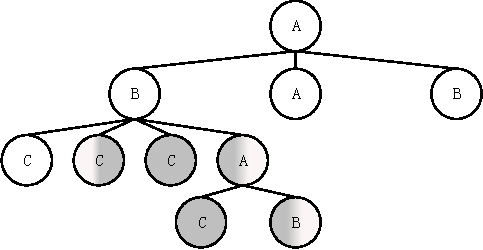
\includegraphics{partialtree/figures/fromWord-1.pdf}
\caption{An example XML tree}
\label{fig:example}
\end{figure}

\begin{figure}[t]
\centering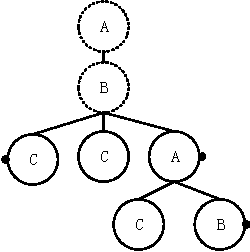
\includegraphics{partialtree/figures/fromWord-3.pdf}
\caption{Partial tree for the example.}
\label{fig:partialtree}
\end{figure}

In this paper, we deal with an important subset of XPath queries called
\emph{navigational XPath queries}~\cite{xpathcategory} in which we specify the nodes with not only
the parent-child relationships but also the inter-sibling relationships
and additional conditions called predicates.  Although a partial tree has
the parent-child relationships from the root, it lacks the information
required to process navigational XPath queries, a node may have only some
of its children, and some siblings may be on another partial tree.
Therefore, we develop a new algorithm for processing navigational XPath
queries over a set of partial trees with communication.
Our algorithm is easy to implement because it processes the steps in a query (including those in predicates) 
one by one and is efficient because we carefully analyzed the conditions to reduce the communication among partial trees.

The contributions of our study are summarized as follows.

\begin{itemize}
\item \textbf{Formalizing the structure for XML chunks}:
We first formalize the structure and properties of partial trees that are given from chunks of an XML document (Section~\ref{sec:partialtree}). We also show an algorithm to parse the chunks and construct the partial trees (Section~\ref{sec:construction}).

\item \textbf{Parallelizing XPath Queries}:
We then develop an algorithm for executing the navigational XPath queries in parallel (Section~5).
Basically, the algorithm runs independently on partial trees, but it also performs communication
to obtain the correct query results.

\item \textbf{Experiments on GB-level XML documents}:
We implemented the algorithm in Java and conducted experiments on a PC cluster with GB-level XML documents (Section~6).  Our implementation successfully processed an 8 GB XML document in parallel and obtained speedups of a factor of 6.0 over 16 PCs.
\end{itemize}


The remainder of the paper is organized as follows. In Section 2, we review the XPath query. In Section 3, we discuss the partial trees in detail. In Section 4, we discuss how to construct partial trees from chunks of an XML document. In Section 5, we discuss executing XPath query  algorithms in parallel. We 
report the experiment results in Section 6. Related work is shown in Section 7, and we conclude the paper in Section 8.


% LocalWords: kmatsu 


\section{XPath Query}

XML path language (XPath)~\cite{XPath} is a W3C standard for representing queries
to XML documents. In XPath, a query is represented in path
notation. In this paper, we focus on an important subset of XPath queries called \emph{navigational XPath queries}~\cite{xpathcategory}. 
Fig.~\ref{fig:grammar} shows the grammar of the XPath queries we use in this paper.

An XPath query in this paper starts from the root and consists of one or more \emph{steps}.
Each step consists of an \emph{axis}, a \emph{name test}, and at most one \emph{predicate}. 
An axis defines a set of nodes relative to the nodes matched for the steps so far.
We can use nine axes
\footnote{%
Since the name-test allows a wildcard ``\texttt{*}'', we can translate the \texttt{following} and \texttt{preceding} axes into a path in the grammar: for example \texttt{following::}$x$ is the same as \texttt{ancestor-or-self::*/}\break\texttt{following-sibling::*/descendant-or-self::}$x$. }

including \verb|following-sibling| and \verb|preceding-sibling|.
A name test is used for selecting nodes: if the name of a tag in an XML document is equal to the name test, the node is selected.  A predicate written 
between ``\verb|[|'' and ``\verb|]|'' describes additional conditions on the matched nodes by using a path without predicates.
For example, ``\verb|/descendant::a/child::b[following-|\break
\verb|sibling::d]|'' is an XPath query with two steps where \verb|descendant| 
and \verb|child| are the axes, \verb|a| and \verb|b| are the name-tests, and a predicate \verb|following-sibling::d| is attached to the second step. 
This query first retrieves all the nodes with name \verb|a| in an XML document, and then among their children it retrieves node \verb|b| with one or more following siblings with name \verb|d|.
In other words, the result of the query is a set of nodes \verb|b| that has its parent \verb|a| and at least one sibling \verb|d| on its right.

\begin{figure}`
\centering\fbox{
\begin{minipage}{.9\linewidth}
\textit{Query} ::= `\texttt{/}' \textit{LocationPath}          \\
\textit{LocationPath} ::= \textit{Step} $~|~$ \textit{Step} `\texttt{/}' \textit{LocationPath}          \\
\textit{Step} ::= \textit{AxisName} `\texttt{::}' \textit{NameTest} \textit{Predicate}?          \\
\textit{AxisName} ::= `\texttt{self}' $~|~$ `\texttt{child}' $~|~$ `\texttt{parent}'          \\
\phantom{\textit{AxisName} :}           $~|~$ `\texttt{descendant}' $~|~$ `\texttt{ancestor}'          \\
\phantom{\textit{AxisName} :}           $~|~$ `\texttt{descendant-or-self}' $~|~$ `\texttt{ancestor-or-self}'          \\
\phantom{\textit{AxisName} :}           $~|~$ `\texttt{following-sibling}' $~|~$ `\texttt{preceding-sibling}'          \\
\textit{NameTest} ::= `\texttt{*}' $~|~$ \textit{string}	          \\
\textit{Predicate} ::= `\texttt{[}' \textit{SimpleLocationPath} `\texttt{]}'          \\
\textit{SimpleLocationPath} ::= \textit{SimpleStep}  \\
\phantom{\textit{SimpleLocationPath} :}           $~|~$ \textit{SimpleStep} `\texttt{/}' \textit{SimpleLocationPath}          \\
\textit{SimpleStep} ::= \textit{AxisName} `\texttt{::}' \textit{NameTest}          
\end{minipage}
}
\caption{Grammars of XPath queries used in this paper}
\label{fig:grammar}
\end{figure}



\section{Partial Tree}
\label{sec:partialtree}

The main idea of our approach for evaluating large XML documents is to 
split an XML document into chunks and query the chunks on different 
computers of a cluster. To support this, we first define the structure for presenting a chunk in
the memory, which is called a \emph{partial tree}.
The partial tree is the core concept in our research. We use partial trees
to represent chunks of an XML document and the XPath queries are also
applied to partial trees. Therefore, to begin with, we will give a
detailed introduction to the partial tree.

\subsection{Node types and definitions}

Partial trees contain many different types of XML nodes.
Four types of nodes are shown in Fig.~\ref{fig:nodetypes}.  A 
closed node has both its start tag and end tag. A node without one of 
its tags is called an open node. A left-open node is missing its start tag, 
and a right-open node is missingits end tag. 
In the figures, the missing tags are illustrated by a black
dot: $\bullet$. A pre-open node is a node missing both of its tags. 
Actually a node is no longer a node if it misses both of its tags. 
But we need it for representing the parent node of a partial tree, 
which specifies the relationships from the root. 
Note that our research focuses on querying nodes; therefore, it is not interesting 
for us that no tag is contained in a chunk, even if we can denote the whole chunk as a pre-open node. 
All the three types of nodes, left-open node, right-open node, or pre-node, are called \emph{open nodes}.
\begin{figure}[t]
	\centering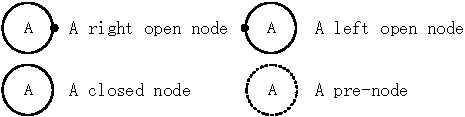
\includegraphics{partialtree/figures/fromWord-2.pdf}
	\caption{Four node types}
	\label{fig:nodetypes}
\end{figure}

\subsection{Standard Model for Partial Tree}

Now we discuss the characteristics that partial trees generally
have. Since the left-open nodes, right-open nodes, and pre-nodes are the special nodes in
partial trees, we focus on the properties of the open node.

The first property is about the parent-child relationship of the open
nodes.

\begin{property}
\label{property1}\itshape
If a node on a partial tree is left/right open, then its parent is also left/right open.
\end{property}

The second property is about the sibling relationship of the open nodes. 

\begin{property}
\label{property2}\itshape
If a node is left open, it is the first node among its
siblings in the partial tree. If a node is right open, it is the last
node among its siblings in the partial tree.
\end{property}

There is another important property of pre-nodes.

\begin{property}
\label{property3}\itshape
If there exist multiple pre-nodes, then only one of
them has left-open/closed/right-open nodes as its child.
\end{property}

We develop a standard model of partial trees  based on these properties
as shown in Fig.~\ref{fig:model}.

\begin{figure}[t]
\centering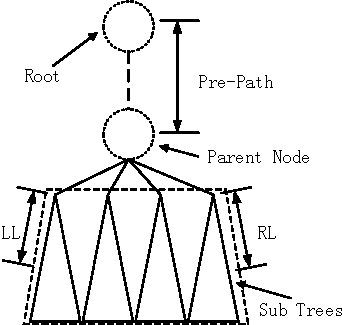
\includegraphics{partialtree/figures/fromWord-4.pdf}
\caption{A standard model of partial tree.}
\label{fig:model}
\end{figure}
 
The partial tree consists vertically of two parts: a list of pre-open
nodes and a forest of subtrees. We call the list of pre-open nodes
\emph{pre-path}. The pre-path plays an important role in applying queries from the root. 
From property~\ref{property3}, one or more subtrees connect to a pre-node at the bottom of
the pre-path. Note that for each subtree, there is only one root, which is
a left-open/closed/right-open node, but there could be one or more subtrees. 

From properties \ref{property1} and \ref{property2}, 
we know that the left-open nodes are located on
the upper-left part of a partial tree and the right-open nodes are located on the
upper-right part. More precisely, the left-open nodes form a list from a
root node of a subtree, and we call the list the \emph{left list} (LL). Likewise, we call the
list of right-open nodes the \emph{right list} (RL). 

%\def\INDEXSET#1{\mathit{#1}_{[0,P)}}
\def\INDEXSET#1{\mathit{#1}_{[P]}}
\def\baselinestretch{1.5}

\section{Partial Tree Construction}
\label{sec:construction}

Since the structure of a partial tree is different from ordinary XML trees, 
we designed an algorithm for partial tree construction.
The algorithm for constructing partial trees has three steps: constructing subtrees from parsing chunks, pre-path computation, and computation for ranges. 

\subsection{Construction of subtrees from parsing XML chunks}

A partial tree is constructed from parsing an input XML chunk, which is  
a substring created from splitting an XML document. We design an algorithm that parses 
the input XML string into a similar tree by using an iterative function with 
a stack. We use an example XML document listed below to demonstrate how our algorithm works.

\begin{quote}\tt\small
<A><B><C><E></E></C><D></D></B><E></E><B><B><D><E>\\
</E></D><C></C></B><C><E></E></C><D><E></E></D></B>\\
<E><D></D></E><B><D></D><C></C></B><B></B></A>\\
\end{quote}
 
From the document, we can create an XML tree as shown in Fig.~\ref{fig:tree}.
We number these nodes in a prefix order for identification.

\begin{figure*}[t]
	\centering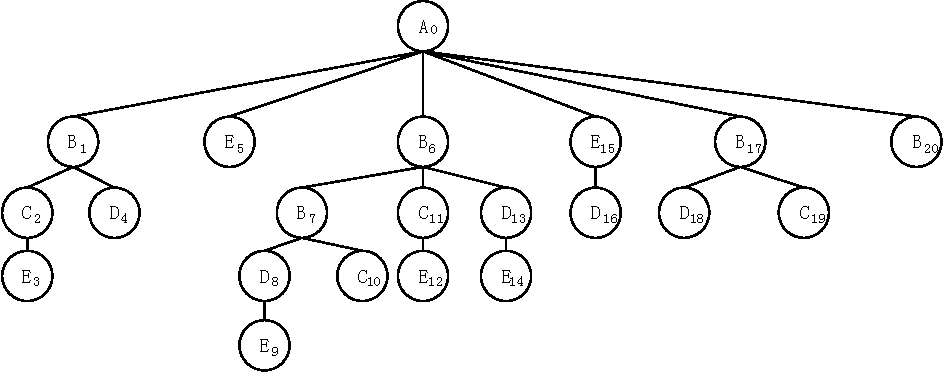
\includegraphics[]{partialtree/figures/fromWord-5.pdf}
	\caption{an XML tree from the given XML string}
	\label{fig:tree}
\end{figure*}

Then, we split the document into five chunks as listed below.

\begin{itemize}
	\item[chunk$_0$:] \texttt{ <A><B><C><E></E></C><D></D></B>}
	\item[chunk$_1$:] \texttt{ <E></E><B><B><D><E></E></D>}
	\item[chunk$_2$:] \texttt{ <C></C></B><C><E></E></C><D>}
	\item[chunk$_3$:] \texttt{ <E></E></D></B><E><D></D></E>}
	\item[chunk$_4$:] \texttt{ <B><D></D><C></C></B><B></B></A>}
\end{itemize}

When splitting an XML document, we need to deal with nodes with missing tags.
During parsing, we push the start tag onto the stack. When we meet an
end tag, we pop the last tag to merge a closed node. However, as a result of splitting, 
some nodes miss their matching tags. In this case, we  
mark it left-open or right-open based on which part is missing. Then, we add them onto 
the subtrees in the same way as we add closed nodes.

We also need to handle the case when the split position falls inside a tag 
and thus splits the tag into two halves.
In this case, we simply merge the split tags. 
Because there are at most two split tags on a partial tree, 
the time taken for merging them is negligible. 

One or more subtrees can be constructed from one chunk.
We construct nine subtrees by parsing the five chunks above as shown in  Fig.~\ref{fig:partialtree-notfinished}.
Chunk$_0$ and chunk$_4$ have only one subtree while chunk$_2$ has three subtrees.
After the parsing phase, these subtrees are used for pre-path computation.

\begin{figure*}[t]
	\centering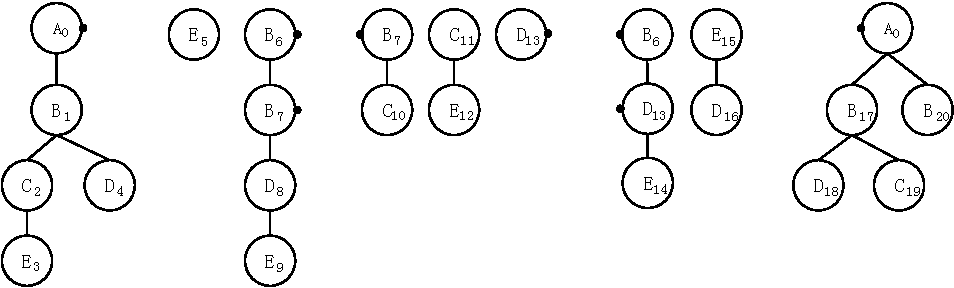
\includegraphics[]{partialtree/figures/fromWord-6.pdf}
	\caption{Subtrees from parsing chunks}
	\label{fig:partialtree-notfinished}
\end{figure*}



\subsection{Pre-path computation}

The basic idea of computing the pre-paths for each partial tree is to 
make use of open nodes, because missing parent and ancestor nodes 
is caused by splitting these nodes. Therefore, the information needed 
for creating the pre-paths lies in these open nodes. 

Algorithm 0 outlined the pseudo codes for pre-path computation. 
Because one chunk may generate more than one subtrees, the input is a list of subtree lists. 
The length of the list is equal to the number of partial trees, thus represent the length as $P$.

Algorithm 0 has three phases.
The first phase selects all left-open nodes to $LLS$ and all right-open nodes to $RLS$ (line 2-4). 
$LLS_{[P]}$ collect the left open nodes of the $p$th partial tree, likewise we have $RLS_{[P]}$.
Note that the nodes in $LLS_{[P]}$ or $RLS_{[P]}$ are arranged in order from root to leaves.
For example, in Table~\ref{table:opennodes}, we select all the open nodes and add them 
to corresponding lists. 
 
 \begin{figure}[t]
 	\centering
 	\label{fig:ppalgorithm}
 	\begin{tabular}{l}
 		\hline
 		\hline
 		\makebox[.95\linewidth][l]{\textbf{Algorithm 0} \textsc{GetPrepath}($\mathit{STS}$)} \\
 		\hline
 		\textbf{Input}: $\mathit{STS}$: a list of subtree lists \\
 		\textbf{Output}: an indexed set of partial trees\\
 		\makebox[1em][r]{1:}\hspace{1 mm} /* open nodes in LLS or RLS are arranged in top-bottom order */\\
 		\makebox[1em][r]{2:}\hspace{1 mm} \textbf{for all} $p \in [0, P)$ \textbf{do} \\
 		\makebox[1em][r]{3:}\hspace{4 mm} $\INDEXSETL{LLS} \leftarrow \mathit{SelectLeftOpenNodes}(\INDEXSETL{STS})$\\
 		\makebox[1em][r]{4:}\hspace{4 mm} $\INDEXSETL{RLS} \leftarrow \mathit{SelectRightOpenNodes}(\INDEXSETL{STS})$\\
 		
 		\makebox[1em][r]{5:}\hspace{1 mm} /* Prepath-computation and collecting matching nodes */\\
 		\makebox[1em][r]{6:}\hspace{1 mm} $AuxList \leftarrow []$ \\
 		\makebox[1em][r]{7:}\hspace{1 mm} \textbf{for} $ p \in [0, P-1) $ \textbf{do}\\
 		\makebox[1em][r]{8:}\hspace{4 mm} $AuxList.\mathit{AppendToHead}(\INDEXSETL{RLS})$\\
 		\makebox[1em][r]{9:}\hspace{4 mm} $AuxList.\mathit{RemoveLast}(LLS_{[p+1]}.\mathit{Size}()) $\\
 		\makebox[1em][r]{10:}\hspace{4 mm} $ PPS_{[p+1]}\leftarrow AuxList$ \\
 		
 		\makebox[1em][r]{11:}\hspace{1 mm}  /* Add pre-nodes to subtrees */ \\
 		\makebox[1em][r]{12:}\hspace{1 mm} $PTS \leftarrow []$ \\
 		\makebox[1em][r]{13:}\hspace{1 mm} \textbf{for} $ p \in [0, P) $ \textbf{do}\\
 		\makebox[1em][r]{14:}\hspace{4 mm} \textbf{for} $ i \in [0, PPS_{[p]}.Size() - 1)$ \textbf{do} \\
 		\makebox[1em][r]{15:}\hspace{8 mm}   $PPS_{[p][i]}.children.$Add$(PPS_{[p][i+1]})$ \\
  		\makebox[1em][r]{16:}\hspace{4 mm} $PPS_{[p]}.last.children.$Add$(\INDEXSETL{STS})$ \\
 		\makebox[1em][r]{17:}\hspace{4 mm}   $\INDEXSETL{PTS} \leftarrow PPS_{[p][0]}$ \\
 		\makebox[1em][r]{18:}\hspace{1 mm} \textbf{return} \emph{PTS} \\
 		\hline
 	\end{tabular}
 \end{figure}

In the second phase, we do the pre-path computation. Once we split an XML document from a position
inside the document, the two partial tree created from splitting have the same number of open nodes 
on the splitting side. Given two consecutive partial trees, the number of right-open nodes of the left partial tree is the same as the number of left-open nodes of the right partial tree. 
We can use this feature to compute pre-paths for partial trees.
We first add the $p$th $RLS$ to the head of an auxiliary list $AuxList$ (line 8), 
then remove the same number of nodes as the number of $(p-1)$th $LLS$ (line 9). 
Last, we keep the nodes in the $AuxList$ to the $(p+1)$th $PPS$, which holds the pre-nodes for each partial tree.
Table~\ref{table:tempresult} shows the results of pre-path computation for the given example.

\begin{table}[t]
	\caption{Open node lists}
	\label{table:opennodes}
	\centering
	\begin{tabular}{c|cc}
		\hline
		& Left-open nodes	& Right-open nodes \\
		\hline
		pt$_0$	& []			& [A$_0$] \\
		pt$_1$	& []			& [B$_6$, B$_7$] \\
		pt$_2$	& [B$_7$]			& [D$_1$$_3$] \\
		pt$_3$	& [B$_6$, D$_1$$_3$]		& [] \\
		pt$_4$	& [A$_0$]			& [] \\
		\hline
	\end{tabular}
\end{table}
 
\begin{table}[t]
	\caption{Results of pre-path computation in AUX}
	\label{table:tempresult}
	\centering
	\begin{tabular}{c|ccc}
		\hline
		& Left-open nodes	& Right-open nodes & $AUX$\\
		\hline
		pt$_0$	& []			& [A$_0$]  & []\\  
		pt$_1$	& []			& [B$_6$, B$_7$] & [A$_0$] \\
		pt$_2$	& [B$_7$]			& [D13] &[A$_0$,B$_6$]\\
		pt$_3$	& [B$_7$, D$_1$$_3$]		& []  & [A$_0$]\\
		pt$_4$	& [A$_0$]			& [] &[]\\
		\hline
	\end{tabular}
\end{table}


In last phase, we add pre-nodes to the corresponding partial tree and copy the nodes in $PPS_{[p]}$ to $PTS_{[p]}$ as results for output.Because pre-nodes in the pre-path are also open nodes, we list all open nodes for each partial trees in Table~\ref{table:allopennodes}. Then, the pre-path computation is complete. For the given example, we obtain the partial trees as shown in Fig.~\ref{fig:partialtree2}.

\begin{table}[t]
	\caption{All open nodes}
	\label{table:allopennodes}
	\centering
	\begin{tabular}{c|cc}
	\hline
	& Left-open nodes	& Right-open nodes \\
	\hline
	pt$_0$	& []						& [A$_0$] \\
	pt$_1$	& [A$_0$]					& [A$_0$, B$_6$, B$_7$] \\
	pt$_2$	& [A$_0$, B$_6$, B$_7$]		& [A$_0$, B$_6$, D$_1$$_3$] \\
	pt$_3$	& [A$_0$, B$_6$, D$_1$$_3$]	& [A$_0$] \\
	pt$_4$	& [A$_0$]					& [] \\
	\hline
	\end{tabular}
\end{table} 


\begin{figure*}[t]
	\centering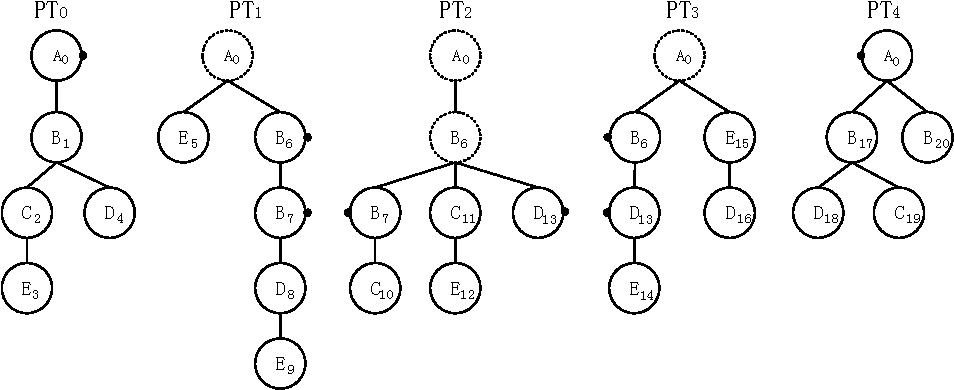
\includegraphics[scale=.9]{partialtree/figures/fromWord-7.pdf}
	\caption{Partial trees from the given XML string.}
	\label{fig:partialtree2}
\end{figure*}

\subsection{Creation of Ranges of Open Nodes}  
Once an XML node is split, it generates two or more open nodes
on consecutive partial trees. For example, as we can see in Fig.~\ref{fig:partialtree2}, 
\Nr{B}{6} on pt$_1$, \Np{B}{6} on pt$_2$, and \Nl{B}{6}  on pt$_3$ 
are created from the same node \Nc{B}{6}.
For locating the open nodes of the same node on different partial trees, 
we use two integers \textit{start} and \textit{end} for the open nodes. With these two integers, 
we can decide the partial trees that have matching nodes of the same open node.
Note that after adding nodes to a partial tree, the nodes from the same node also have the 
same depth. Therefore, we can locate all the matching nodes to set \textit{start} and \textit{end} for each open node. 
After computation, we obtain the ranges shown in Table~\ref{table:rangesresult}. 

\begin{table}[t]
	\caption{Open node lists with ranges}
	\label{table:rangesresult}
	\centering
	\begin{tabular}{c|cc}
		\hline
		& Left open nodes	& Right open nodes \\
		\hline
		pt$_0$	& []	& [A$_0$(0,4)] \\
		pt$_1$	& [A$_0$(0,4)]	& [A$_0$(0,4), B$_6$(1,3), B$_7$(1,2)] \\
		pt$_2$	& [A$_0$(0,4), B$_6$(1,3), B$_7$(1,2)]	& [A$_0$(0,4), B$_6$(1,3), D$_1$$_3$(2,3)] \\
		pt$_3$	& [A$_0$(0,4), B$_6$(1,3), D$_1$$_3$(2,3)]	& [A$_0$(0,4)] \\
		pt$_4$	& [A$_0$(0,4)]	& [] \\
		\hline
	\end{tabular}
\end{table}

By using these ranges, we can locate the matching nodes of the same node on the different partial trees.
For example, the range of A$_0$ is (0, 4), that means we can 
locate the same nodes of \Nc{A}{0} from pt$_0$ to pt$_4$.
As we can see, there are \Nr{A}{0}, \Np{A}{0}, \Np{A}{0}, 
\Np{A}{0}, and \Nr{A}{0} on pt$_0$ to pt$_4$, respectively.


% LocalWords: fromWord pdf subtree subtrees pre


\section{XPath Queries on Partial Trees}

When we design the XPath query algorithms for a set of partial trees, there are the following three main difficulties.

First, a node in the original XML tree may be split into two or more nodes in different partial trees.
When such a node is selected in a partial tree (e.g., \Nr{B}{6} on \PT1), the other corresponding nodes (\Np{B}{6} on \PT2 and \Nl{B}{6} on \PT3) should also be selected to be consistent.

Second, though the partial trees have all the parent-child edges of their nodes, 
the sibling-relation that is split among partial trees is missing.
When we perform queries with \texttt{following-sibling} or \texttt{preceding-sibling},
the results may be on another (possibly far) partial tree.
We need to design an algorithm to let the partial trees know about such cases.

Third, when we perform queries with a predicate, we usually execute the sub-query in the predicate
from a set of matching nodes.  However, on a set of partial trees, the starting nodes and the matching nodes 
of the sub-query may be on different partial trees.
We also need an algorithm to propagate the information over partial trees for queries with predicates.

In this section, we develop an algorithm for XPath queries on a set of partial trees.
We first show the outline of the algorithm and then describe the details of the queries.
We use the following three XPath expressions
as our running examples.
\begin{itemize}
\item [Q1]: \texttt{\small /child::A/descendant::B/descendant::C/parent::B}
\item [Q2]: \texttt{\small /descendant::B/following-sibling::B}
\item [Q3]: \texttt{\small /descendant::B[following-sibling::B/child::C]\\/child::C}
\end{itemize}
We also discuss the complexity of our algorithm at the end of this section.

%% Our objective is to design an easy-to-implement and highly
%% efficient way of querying GB-level XML documents in parallel. 
%% The difficulty of evaluation of XPath queries on partial trees
%% is mainly caused by the distributed structure information of XML documents. 
%% If we apply XPath queries to a partial tree in the same way 
%% as querying on an ordinary XML tree, we cannot collect all the results 
%% without structure information of the other partial trees. 
%% Some XPath queries also depend on the structure information of partial trees, 
%% for example we cannot select all the following siblings of a node 
%% if some of its following siblings are located on other partial trees. 
%% Therefore, we need to use the information stored in the global area, 
%% which contains the structure information of open nodes of all the partial trees.

%% The difficulty of XPath querying on partial trees in parallel is due to the
%% missing the structure information of the other partial trees. 
%% The splitting generates many open nodes, which are the key point of designing the algorithm
%% for applying XPath queries on partial trees.
%% Therefore, we are mainly concerned with how to process the open nodes.
%% In our study, open nodes are more important and useful during the querying, 
%% when more than two nodes correspond to the same node. 
%% During the queries, if an open node is selected after the evaluation of a step, 
%% the open nodes corresponding to the same node should also be selected. 
%% For example, when \Nr{B}{7} on \PT1 in Fig.~\ref{fig:partialtree2} is selected, 
%% \Np{B}{7} on \PT2 and \Nl{B}{7} on \PT3 should be selected as well.
%% Therefore, one question of evaluating queries is how to determine
%% which partial trees contain the open nodes that from the same node. 
%% Since we have defined ranges in the open nodes in a global area, 
%% we can use them for solving this question.   
\subsection{Node Definition}

We give a few definitions to partial tree nodes for XPath queries. Each node has a \textit{type} denoting its node type and \textit{depth} 
 denoting the number of edges from the node to the root. 
 A node has four pointers pointing to related nodes: the \textit{parent} pointer points to its parent 
 and the \textit{children} pointer points to its children. For accessing siblings, it has the \textit{presib} pointer 
 and the \textit{folsib} pointer that point to its preceding-sibling node and following-sibling node, respectively.  
It is a common requirement that we should know from which partial tree a node comes in distributed 
 memory environments; therefore, we number each partial tree with a unique id denoted as \textit{partial tree id} or 
 simply \textit{ptid} for distinguishing partial trees. We number \textit{ptid} from 0 to \textit{P - 1} 
 (where P is the total number of partial trees) in document order. 
 Each node has a unique id called \textit{uid}, and we define data type \textit{Link} for holding ptid and uid. 
 By using \textsc{FindNode}(\textit{pt}, \textit{uid}), we can locate any node with a unique integer uid on partial tree \textit{pt}. 
 We assume that we can find a node in constant time.  
 
\subsection{Queries without Predicate}

Algorithm~1 shows the outline of our XPath query algorithm.
The inputs are a query and a set of partial trees.
The output is a set of matching nodes, each of which is associated with the corresponding partial tree.

The query starts from the root of the XML tree.
Note that the root node corresponds to the root node of every partial tree,
and they are put into the lists for intermediate results (lines 1--2).
Hereafter, the loops by $p$ over $[0, P)$ are assumed to be executed in parallel.

An XPath query consists of one or more steps, and in our algorithm
they are processed one by one.  For each step, our algorithm calls
a sub-algorithm based on its axis (given later) and updates the intermediate results (line 4).

Lines 6--9 will be executed when a query has a predicate.
We will explain this part later in Section~5.3.


%% An XPath step consists of one or more steps. We evaluate the
%% steps of an XPath expression in a sequential order from the left to
%% right. For each step, we first deal with axis which determines the
%% relationship of the result nodes to the test node. Then we evaluate
%% the node to select the nodes that satisfy the node test. As we can see
%% in Algorithm 1, We run queries on \textit{P} partialt trees.
%% Note that the loop can be executed in parallel(line X), so are the following algorithms
%% In the loop, we start an XPath query from the roots of partial trees(line 3).
%% We run the query on all the partial trees in parallel. The intermediate results of each step 
%% are stored in a local result list (line 6).  
%% When the evaluation process for one step is over, it produces a new node set that contains the nodes 
%% satisfying the current step. Then the result list is cleared and added with the latest results. 
%% The results of a step are the inputs of the following step. After last step is done,  
%% the result list hold the final results.
%% For the steps in predicates, we first copy nodes from result lists to 
%% predicate result lists (line 8) and create links for each node by \textsc{PreparePredicate}(Lists).
%% Then, we evaluate steps the same as ordinary steps and collect the results computed from each steps (line 9-10).
%% After all the steps in a predicate are evaluated, we call \textsc{ProcessPredicate}(Lists) to process results (line 11).
%% And then return the final result lists.


\begin{figure}[t]
	\centering
	\begin{tabular}{l}
		\hline
		\hline
		\makebox[.95\linewidth][l]{\textbf{Algorithm 1} \textsc{Query}($\mathit{steps}$, $\INDEXSET{pt}$)} \\
		\hline
		\textbf{Input}:           $\mathit{steps}$: an XPath expression \\
                \phantom{\textbf{Input}:} $\INDEXSET{pt}$: an indexed set of partial trees \\
		\textbf{Output}: an indexed set of results of query \\
		\makebox[1em][r]{1:}\hspace{1 mm} \textbf{for} $p \in [0, P)$ \textbf{do} \\
		\makebox[1em][r]{2:}\hspace{4 mm}    $\mathit{ResultList}_p \leftarrow \{~ \mathit{pt}_p.\mathit{root} ~\}$ \\
		\makebox[1em][r]{3:}\hspace{1 mm} \textbf{for all} $\emph{step} \in \emph{steps}$ \textbf{do} \\
		\makebox[1em][r]{4:}\hspace{4 mm}    $\INDEXSET{ResultList}$ \\
                \makebox[1em][r]{  }\hspace{6 mm}        ${}\leftarrow \hbox{\textsc{Query}}\langle\mathit{step}.\mathit{axis}\rangle(\INDEXSET{pt}, \INDEXSET{ResultList}, \mathit{step}.\mathit{test})$ \\
		\makebox[1em][r]{5:}\hspace{4 mm}    \textbf{if} $step.predicate \neq \hbox{\textsc{null}}$ \textbf{then} \\
		\makebox[1em][r]{6:}\hspace{7 mm}       $\INDEXSET{PResultList} \leftarrow \hbox{\textsc{PreparePredicate}}(\INDEXSET{ResultList})$ \\
		\makebox[1em][r]{7:}\hspace{7 mm}       \textbf{for all} $\emph{pstep} \in \emph{step.predicate}$ \textbf{do} \\
		\makebox[1em][r]{8:}\hspace{10 mm}         $\INDEXSET{PResultList}$ \\
                \makebox[1em][r]{  }\hspace{12 mm}             ${} \leftarrow  \hbox{\textsc{PQuery}}\langle\mathit{step}.\mathit{axis}\rangle(\INDEXSET{pt}, \INDEXSET{PResultList}, \mathit{pstep})$ \\
		\makebox[1em][r]{9:}\hspace{7 mm}       $\INDEXSET{ResultList} \leftarrow \hbox{\textsc{ProcessPredicate}}(\INDEXSET{PResultList})$ \\
		\makebox[1em][r]{10:}\hspace{1 mm} \textbf{return} $\INDEXSET{ResultList}$ \\
		\hline
	\end{tabular}
        \caption{Overall algorithm of XPath query for partial trees}
	\label{fig:algQuery2}
\end{figure}
%% \begin{figure}[t]
%% 	\centering
%% 	\label{fig:algQuery}
%% 	\begin{tabular}{l}
%% 		\hline
%% 		\textbf{Algorithm 1} \textsc{Query} (\emph{steps}, \emph{pts}) \\
%% 		\hline
%% 		\textbf{Input}: an XPath expression \emph{steps}, all partial trees \emph{pts} \\
%% 		\textbf{Output}: results of query  \\
%% 		~1: \hspace{1 mm} $ResultLists \leftarrow []$ \\
%% 		~2: \hspace{1 mm} \textbf{for} $p \in [0, P)$ \textbf{do} \\
%% 		~3: \hspace{4 mm} $ResultLists[p]$.Add($pt_p.root$) \\
%% 		~4: \hspace{1 mm} \textbf{for all} $\emph{step} \in \emph{steps}$ \textbf{do} \\
%% 		~5: \hspace{4 mm} SetIsChecked$(pts[p], \mathit{false})$ \\
%% 		~6: \hspace{4 mm} \emph{ResultLists} $ \leftarrow $ Query$<$\emph{Step}.axis$>$(\emph{ResultLists}, \emph{step})\\
%% 		~7: \hspace{4 mm} \textbf{if} $step.predicate \neq NULL$ \textbf{then} \\
%% 		~8: \hspace{8 mm} \emph{PResultLists} $\leftarrow$ \textsc{PreparePredicate}(\emph{ResultLists}) \\
%% 		~9: \hspace{8 mm} \textbf{for all} $\emph{pstep} \in \emph{step.predicate}$ \textbf{do} \\
%% 		10: \hspace{12 mm} \emph{PResultLists}$ \leftarrow $ \textsc{QueryPredicate}$<$\emph{step.axis}$>$ \\
%% 		\hspace{4 mm} (\emph{PResultLists}, \emph{pstep}) \\
%% 		11: \hspace{3 mm} \emph{ResultLists} $ \leftarrow $ \textsc{ProcessPredicate}(\emph{PResultLists})  \\
%% 		12: \hspace{0 mm} \textbf{return} \emph{ResultLists} \\
%% 		\hline
%% 	\end{tabular}
%% \end{figure}

\subsubsection{Downwards Axes}

Algorithm 2 shows the procedure for querying a step with a child axis. 
The input $\INDEXSET{InputList}$ has the nodes selected up to the last step on each partial tree.
The algorithm simply lists up all the children of input nodes and compares their tags with the node test (lines 3--4).

Algorithm 3 shows the procedure for querying a step with descendant axis.
Starting from every node in the input, we traverse the partial tree by 
depth-first search with a stack. 
To avoid traversing the same node more than once, we add the $\mathit{isChecked}$ flag for each node (lines 8--9).
Note that we can reduce the worst-case complexity using this flag from square to linear with respect to the number of nodes.

\begin{figure}[t]
	\centering
	\begin{tabular}{l}
		\hline
		\hline
		\makebox[.95\linewidth][l]{\textbf{Algorithm 2} \textsc{Query}$\langle$\texttt{child}$\rangle$($\INDEXSET{pt}$, $\INDEXSET{InputList}$, $\mathit{test}$)} \\
		\hline
		\textbf{Input}:           $\INDEXSET{pt}$: an indexed set of partial trees \\
                \phantom{\textbf{Input}:} $\INDEXSET{InputList}$: an indexed set of input nodes \\
                \phantom{\textbf{Input}:} $\mathit{test}$: a string of nametest \\
		\textbf{Output}: an indexed set of results \\
		\makebox[1em][r]{1:}\hspace{1 mm} \textbf{for} $p \in [0, P)$ \textbf{do} \\
		\makebox[1em][r]{2:}\hspace{4 mm}    $\mathit{OutputList}_p \leftarrow [] $ \\
		\makebox[1em][r]{3:}\hspace{4 mm}    \textbf{for all} $n \in InputList_p$ \textbf{do} \\
		\makebox[1em][r]{4:}\hspace{7 mm}       $\mathit{OutputList}_p $ \\
                \makebox[1em][r]{  }\hspace{9 mm}          ${}\leftarrow \mathit{OutputList}_p \cup [nc ~|~ nc \in n.\mathit{children}, nc.\mathit{tag} = \mathit{test}] $ \\
		\makebox[1em][r]{5:}\hspace{1 mm} \textbf{return} $\INDEXSET{OutputList}$ \\
		\hline
                \\
		\hline
		\hline
		\makebox[.95\linewidth][l]{\textbf{Algorithm 3} \textsc{Query}$\langle$\texttt{descendant}$\rangle$($\INDEXSET{pt}$, $\INDEXSET{InputList}$, $\mathit{test}$)} \\
		\hline
		\textbf{Input}:           $\INDEXSET{pt}$: an indexed set of partial trees \\
                \phantom{\textbf{Input}:} $\INDEXSET{InputList}$: an indexed set of input nodes \\
                \phantom{\textbf{Input}:} $\mathit{test}$: a string of nametest \\
		\textbf{Output}: an indexed set of results \\
		\makebox[1em][r]{1:}\hspace{1 mm} \textbf{for} $p \in [0, P)$ \textbf{do} \\
		\makebox[1em][r]{2:}\hspace{4 mm}    $\mathrm{SetIsChecked}(\mathit{pt}_p, \mathit{false})$ \\
		\makebox[1em][r]{3:}\hspace{4 mm}    $\mathit{OutputList} \leftarrow [] $ \\
		\makebox[1em][r]{4:}\hspace{4 mm}    \textbf{for all} $n \in InputList_p$ \textbf{do} \\
		\makebox[1em][r]{5:}\hspace{7 mm}       $\mathit{Stack} \leftarrow \{ \emph{n} \}$ \\
		\makebox[1em][r]{6:}\hspace{7 mm}       \textbf{while not }$\mathit{Stack}.\mathit{Empty()}$ \textbf{do}  \\
		\makebox[1em][r]{7:}\hspace{10mm}         $nt \leftarrow \mathit{Stack}.\mathit{Pop}()$  \\
		\makebox[1em][r]{8:}\hspace{10mm}         \textbf{if} $nt.\mathit{isChecked}$ \textbf{then} \textbf{continue} \\
		\makebox[1em][r]{9:}\hspace{10mm}         $nt.\mathit{isChecked} \leftarrow \hbox{\textsc{true}}$ \\
		\makebox[1em][r]{10:}\hspace{10mm}         $\mathit{OutputList}_p $ \\
                \makebox[1em][r]{   }\hspace{12mm}             ${}\leftarrow \mathit{OutputList}_p \cup [nc ~|~ nc \in nt.children, nc.\mathit{tag} = \mathit{test}] $ \\
		\makebox[1em][r]{11:}\hspace{10mm}         $\mathit{Stack}.\mathit{PushAll}(nt.\mathit{children})$ \\
		\makebox[1em][r]{12:}\hspace{1 mm} \textbf{return} $\INDEXSET{OutputList}$ \\
		\hline
	\end{tabular}
        \caption{Query algorithm for downwards axes}
	\label{fig:algQueryChild2}
\end{figure}
%% \begin{figure}[t]
%% 	\centering
%% 	\label{fig:algQueryChild}
%% 	\begin{tabular}{l}
%% 		\hline
%% 		\textbf{Algorithm 2} \textsc{Query}$<$Child$>$ (\emph{InputLists}, \emph{test}) \\
%% 		\hline
%% 		\textbf{Input}: input node lists to be tested \emph{InputLists}, a name test \emph{test} \\
%% 		\textbf{Output}: a list of result lists  \\
%% 		~1: \hspace{1 mm} $\mathit{OutputList} \leftarrow [] $ \\
%% 		~2: \hspace{1 mm} \textbf{for} $p \in [0, P)$ \textbf{do} \\
%% 		~3: \hspace{4 mm} \textbf{for all} $n \in InputLists[p]$ \textbf{do} \\
%% 		~4: \hspace{8 mm} \textbf{for all} $nc \in n.children$ \textbf{do} \\
%% 		~5: \hspace{12 mm} \textbf{if} $nc.tag = test$ \textbf{then}  \\
%% 		~6: \hspace{16 mm} $OutputLists[p]$.Add(\emph{nc})   \\
%% 		~7: \hspace{1 mm} \textbf{return} \emph{OutputLists} \\
%% 		\hline
%% 		\hline
%% 		\textbf{Algorithm 3} \textsc{Query}$<$Descendant$>$ (\emph{InputLists}, \emph{test}) \\
%% 		\hline
%% 		\textbf{Input}:  node lists to be tested \emph{InputLists}, a name test \emph{test} \\
%% 		\textbf{Output}: a list of result lists  \\
%% 		~1: \hspace{1 mm} $\mathit{OutputList} \leftarrow [] $ \\
%% 		~2: \hspace{1 mm} \textbf{for} $p \in [0, P)$ \textbf{do} \\
%% 		~3: \hspace{4 mm} \textbf{for all} $n \in InputLists[p]$ \textbf{do} \\
%% 		~4: \hspace{8 mm} \emph{Stack}.Push(\emph{n}) \\
%% 		~5: \hspace{8 mm} \textbf{while not}(\emph{Stack}.Empth()) \textbf{do}  \\
%% 		~6: \hspace{12 mm} $nt \leftarrow Stack$.Pop()  \\
%% 		~7: \hspace{12 mm} \textbf{if} $nt.isChecked = true$ \textbf{then} \emph{continue} \\
%% 		~8: \hspace{12 mm} $nt.isChecked \leftarrow true$ \\
%% 		~9: \hspace{12 mm} \textbf{for all} $n \in nt.children$ \textbf{do} \\
%% 		10: \hspace{16 mm} \textbf{if} $nc.tag = test$ \textbf{then} \\
%% 		11: \hspace{20 mm} $OutputLists[p]$.Add(\emph{nc}) \\
%% 		12: \hspace{16 mm} $\mathit{Stack}$.Puch($nc$) \\
%% 		13: \hspace{0 mm} \textbf{return} \emph{OutputLists} \\
%% 		\hline
%% 	\end{tabular}
%% \end{figure}

Now let us look at our running example Q1.
For the first step \texttt{child::A}, we obtain only one node for each partial tree.
%
\begin{center}\small
\medskip
\begin{tabular}{ccccc}
\hline
\hline
\PT0 & 
\PT1 &
\PT2 &
\PT3 &
\PT4 \\
\hline
$ [\Nr{A}{0}] $ &
$ [\Np{A}{0}] $ &
$ [\Np{A}{0}] $ &
$ [\Np{A}{0}] $ &
$ [\Nl{A}{0}] $ \\
\hline
\end{tabular}
\medskip
\end{center}
%\texttt{\small pt$_0$ to pt$_4$: [\Nr{A}{0}] [\Np{A}{0}] [\Np{A}{0}] [\Np{A}{0}] [\Nl{A}{0}]}
%
Then we perform the next step \texttt{descendant::B} independently for each partial tree 
from the result shown above.  The following are the results up to \texttt{descendant::B}.
%
\begin{center}\small
\medskip
\begin{tabular}{ccccc}
\hline
\hline
\PT0 & 
\PT1 &
\PT2 &
\PT3 &
\PT4 \\
\hline
$ [\Nc{B}{1}] $ &
$ [\Nr{B}{6}, \Nr{B}{7}] $ &
$ [\Np{B}{6}, \Nl{B}{7}] $ &
$ [\Nl{B}{6}] $ &
$ [\Nc{B}{17}, \Nc{B}{20}] $ \\
\hline
\end{tabular}
\medskip
\end{center}
%
For the third step \texttt{descendant::C}, the algorithm works in a similar way.
It is worth noting that the $\mathit{isChecked}$ flag now works.
For example, on \PT1, starting from \Nr{B}{6}, we traverse \Nr{B}{7}, \Nc{D}{8}, \Nc{E}{9},
and then starting from \Nr{B}{7}, we can stop the traverse immediately.
The results up to \texttt{descendant::C} are as follows.
%
\begin{center}\small
\medskip
\begin{tabular}{ccccc}
\hline
\hline
\PT0 & 
\PT1 &
\PT2 &
\PT3 &
\PT4 \\
\hline
$ [\Nc{C}{2}] $ &
$ [\,] $ &
$ [\Nc{C}{10}, \Nc{C}{11}] $ &
$ [\,] $ &
$ [\Nc{C}{19}] $ \\
\hline
\end{tabular}
\medskip
\end{center}
	
\subsubsection{Upwards Axes}

In the querying of a step with downwards axes, the algorithm has nothing
specific to partial trees.  This is due to Property 1 in Section 3.2.
Let an open node $x$ be selected after a downwards query. Then, it should have started
from an open node (this is an ancestor of $x$) and the corresponding nodes should have all been selected,
which means all the nodes corresponding to $x$ should be selected after the query.

This discussion does not hold for the queries with an upwards axis.
When an open node is selected after an upwards query, it may come from a closed node and
we have no guarantee that all the corresponding open nodes are selected.
Therefore, we add a postprocessing of sharing the selected nodes for the upwards axes.

Algorithm 4 shows the procedure for querying a step with parent axis.
It has almost the same flow as that of the child axis (lines 1--5),
except for the last call of the \textsc{ShareNodes} function.

The \textsc{ShareNodes} function keeps open node consistency.
It consists of two parts\footnote{In our implementation of this \textsc{ShareNodes} function, there are two phases of communication:
all the partial trees send their open nodes to a process and then the necessary data
for a partial tree are sent back.
}.
First, it collects all the selected open nodes from partial trees (lines 4--6).
Then, based on the range information of node $n$ ($n.\mathit{start}$ and $n.\mathit{end}$),
we add all the corresponding selected nodes to all the partial trees.

Now, we continue our running example Q1. For the \texttt{parent::B} after the \texttt{descendant::C},
we first directly select the parent nodes of the intermediate results independently.
The results are as follows.
%
\begin{center}\small
\medskip
\begin{tabular}{ccccc}
\hline
\hline
\PT0 & 
\PT1 &
\PT2 &
\PT3 &
\PT4 \\
\hline
$ [\Nc{B}{1}] $ &
$ [\,] $ &
$ [\Nl{B}{7}, \Np{B}{6}] $ &
$ [\,] $ &
$ [\Nc{B}{17}] $ \\
\hline
\end{tabular}
\medskip
\end{center}
%
Here, unfortunately node \Nl{B}{7} is selected on \PT2, but its corresponding node on \PT1 is not selected.

We then compute the \textsc{ShareNodes} function.
By collecting all the open nodes from all the partial trees, we have a list $[\Nl{B}{7}, \Np{B}{6}]$.
Since they have ranges $(1, 2)$ and $(1, 3)$, respectively, \PT1 receives two nodes \Nr{B}{7} and \Nr{B}{6},
\PT2 receives two nodes \Nl{B}{7} and \Np{B}{6}, and \PT3 receives one node \Nl{B}{6}.
By taking the union with the previous intermediate results, we obtain the following final results.

\begin{center}\small
\medskip
\begin{tabular}{ccccc}
\hline
\hline
\PT0 & 
\PT1 &
\PT2 &
\PT3 &
\PT4 \\
\hline
$ [\Nc{B}{1}] $ &
$ [\Nr{B}{6}, \Nr{B}{7}] $ &
$ [\Nl{B}{7}, \Np{B}{6}] $ &
$ [\Nl{B}{6}] $ &
$ [\Nc{B}{17}] $ \\
\hline
\end{tabular}
\medskip
\end{center}
% \texttt{\small pt$_0$ to pt$_4$: [B$_1$]	[B$_6$+, B$_7$+]	[+B$_7$, \Np{B}{6}]	[+B$_6$]	[B$_{17}$]}

\begin{figure}[t]
	\centering
	\begin{tabular}{l}
		\hline
		\hline
		\makebox[.95\linewidth][l]{\textbf{Algorithm 4} \textsc{Query}$\langle$\texttt{parent}$\rangle$($\INDEXSET{pt}$, $\INDEXSET{InputList}$, $\mathit{test}$)} \\
		\hline
		\textbf{Input}:           $\INDEXSET{pt}$: an indexed set of partial trees \\
                \phantom{\textbf{Input}:} $\INDEXSET{InputList}$: an indexed set of input nodes \\
                \phantom{\textbf{Input}:} $\mathit{test}$: a string of nametest \\
		\textbf{Output}: an indexed set of results \\
		\makebox[1em][r]{1:}\hspace{1 mm} \textbf{for} $p \in [0, P)$ \textbf{do} \\
		\makebox[1em][r]{2:}\hspace{4 mm}    $\mathit{OutputList}_p \leftarrow [\,]$ \\
		\makebox[1em][r]{3:}\hspace{4 mm}    \textbf{for all} $n \in \mathit{InputList}_p$ \textbf{do} \\
		\makebox[1em][r]{4:}\hspace{7 mm}       \textbf{if} $n.\mathit{parent} \neq \hbox{\textsc{null}}$ \textbf{ and } $n.\mathit{parent}.\mathit{tag} = \emph{test}$ \textbf{then} \\
		\makebox[1em][r]{5:}\hspace{10mm}          $\mathit{OutputList}_p.\mathit{Add}(n)$ \\
		\makebox[1em][r]{6:}\hspace{1 mm} \textbf{return} \textsc{ShareNodes}($\INDEXSET{pt}$, $\INDEXSET{OutputList}$) \\
		\hline
                \\
                \hline
		\hline
		\makebox[.95\linewidth][l]{\textbf{Algorithms 5} \textsc{ShareNodes}($\INDEXSET{pt}$, $\INDEXSET{NodeList})$} \\
		\hline
		\textbf{Input}:           $\INDEXSET{pt}$: an indexed set of partial trees \\
                \phantom{\textbf{Input}:} $\INDEXSET{NodeList}$: an indexed set of nodes \\
		\textbf{Output}: an indexed set of nodes after sharing\\
		\makebox[1em][r]{1:}\hspace{1 mm} /* Select all open nodes and append them to a node list */ \\
		\makebox[1em][r]{2:}\hspace{1 mm} $\mathit{ToBeShared} \leftarrow [\,]$ \\
		\makebox[1em][r]{3:}\hspace{1 mm} \textbf{for} $p \in [0, P)$ \textbf{do} \\
		\makebox[1em][r]{4:}\hspace{4 mm} $ \mathit{OpenNodes} \leftarrow [n ~|~ n \in \mathit{NodeList}_p, $\\
		\makebox[1em][r]{5:}\hspace{4 mm} \phantom{$ \mathit{OpenNodes} \leftarrow [n ~|~$}$n.\mathit{type} \in \{\textsc{LeftOpen}, \textsc{RightOpen}, \textsc{PreNode}\}]$\\
		\makebox[1em][r]{6:}\hspace{4 mm} $ \mathit{ToBeShared} \leftarrow \mathit{ToBeShared} \cup \mathit{OpenNodes}$ \\[5pt]
		\makebox[1em][r]{7:}\hspace{1 mm} /* Regroup nodes by partial tree id and add them to NodeList */ \\
		\makebox[1em][r]{8:}\hspace{1 mm} \textbf{for} $p \in [0, P)$ \textbf{do} \\
		\makebox[1em][r]{9:}\hspace{4 mm}    $\mathit{ToBeAdded}_p \leftarrow [n ~|~ n \in \mathit{ToBeShared}, n.\mathit{start} \le p \le n.\mathit{end}]$ \\
		\makebox[1em][r]{10:}\hspace{4 mm}    $\mathit{OutputList}_p \leftarrow \mathit{NodeList}_p \cup \mathit{ToBeAdded}_p$ \\
		\makebox[1em][r]{11:}\hspace{1 mm} \textbf{return} $\INDEXSET{OutputList}$ \\ 
		\hline 
	\end{tabular}
        \caption{Query algorithms for upwards axes}
	\label{fig:algQueryParent2}
\end{figure}	
%% \begin{figure}[t]
%% 	\centering
%% 	\label{fig:algQueryChild}
%% 	\begin{tabular}{l}
%% 		\hline
%% 		\textbf{Algorithm 4} \textsc{Query}$<$Parent$>$ (\emph{InputLists}, \emph{test}) \\
%% 		\hline
%% 		\textbf{Input}: a list of node lists \emph{InputLists}, a name test \emph{test} \\
%% 		\textbf{Output}: a list of node lists  \\
%% 		~1: \hspace{1 mm} $\mathit{OutputList} \leftarrow [] $ \\
%% 		~2: \hspace{1 mm} \textbf{for} $p \in [0, P)$ \textbf{do} \\
%% 		~3: \hspace{4 mm} \textbf{for all} $n \in InputLists[p]$ \textbf{do} \\
%% 		~4: \hspace{8 mm} \textbf{if} $n.parent \neq NULL \textbf{ and } n.parent = \emph{test}$ \textbf{then} \\
%% 		~5: \hspace{12 mm} \emph{OutputLists}[$p$].Add($n$) \\
%% 		~6: \hspace{0 mm} \textbf{return} \emph{OutputLists} \\
%% 		\hline
%% 		\hline
%% 		\textbf{Algorithms 5} \textsc{ShareNodes}(\emph{pts}, \emph{NodeLists}) \\
%% 		\hline
%% 		\textbf{Input}: all partial trees \emph{pts}, the node lists that need to share \emph{NodeLists} \\
%% 		\textbf{Output}: the node lists after sharing\\
%% 		~1: \hspace{1 mm} $\mathit{ShareLists} \leftarrow []$ \\
%% 		~2: \hspace{1 mm} /* Select all open nodes and append to a node list */ \\
%% 		~3: \hspace{1 mm} \textbf{for} $p \in [0, P)$ \textbf{do} \\
%% 		~4: \hspace{4 mm} $ \mathit{OpenNodes} \leftarrow \{n | n \in \mathit{NodeLists}[p], n.type \in \{\textsc{LeftOpen, RightOpen}\}\}$\\
%% 		~5: \hspace{4 mm} $ \mathit{ShareNodes} \leftarrow \mathit{ShareNodes} \cup \mathit{OpenNodes}$ \\
%% 		~6: \hspace{1 mm} /* Regroup nodes by partial tree id */ \\
%% 		~7: \hspace{1 mm} \textbf{for} $\emph{n} \in \emph{ShareNodes}$ \textbf{do} \\
%% 		~8: \hspace{4 mm} \textbf{for} $i \in [n.\mathit{start}, n.\mathit{end})$ \textbf{do} \\
%% 		~9: \hspace{8 mm} \emph{ShareLists}[\emph{i}].Add(\emph{n}) \\
%% 		10: \hspace{1 mm} /* Add corresponding nodes to NodeLists */\\
%% 		11: \hspace{1 mm} \textbf{for} $p \in [0, P)$ \textbf{do} \\
%% 		12: \hspace{4 mm}  $\mathit{ResultLists}[p] \leftarrow \mathit{ResultLists} \cup \mathit{ShareLists}[p]$ \\
%% 		13: \hspace{1 mm} \textbf{return} \emph{NodeLists} \\ 
%% 		\hline 
%% 	\end{tabular}
%% \end{figure}	


\subsubsection{Intra-sibling Axes}

The following- or preceding-sibling axes retrieve nodes from a set of nodes
that are siblings of an intermediate node.  In our partial trees, a set of those sibling nodes
might be divided into two or more partial trees. 
Therefore, these intro-sibling axes require querying on other partial trees in addition to the local querying.

Without loss of generality, we discuss the following-sibling axis only.
Algorithm 6 shows the procedure for querying a step of following-sibling axis,
which consists of four stages: local query, preparation, regrouping, and remote query.

In the local query, we utilize the $\mathit{folsib}$ pointer and the $\mathit{isChecked}$ flag
to realize linear-time querying (lines 6--10). 
Then, in the preparation, we select the nodes that are passed to another partial tree
to perform the remote query.  The latter two conditions (lines 14, 15) are rather easy:
we will ask a remote query if the parent node can have more segments on the right (i.e., right open).
The former condition (line 13) is a little tricky.  Even if the latter two conditions hold,
we do not need a remote query if the node itself is right open.  Notice that if a node is right open
then it should have a corresponding left-open node on another partial tree, and 
that node will ask for a remote query.  The regrouping is almost the same as that in \textsc{ShareNodes},
and the difference is the range we consider (we only look at the right for the following-sibling).
Finally, the remote query finds the children from the intermediate nodes given by regrouping.

Now, let us look at our running example Q2.
After \texttt{descendant::B}, we have the following results.
%
\begin{center}\small
\medskip
\begin{tabular}{ccccc}
\hline
\hline
\PT0 & 
\PT1 &
\PT2 &
\PT3 &
\PT4 \\
\hline
$ [\Nc{B}{1}] $ &
$ [\Nr{B}{6}, \Nr{B}{7}] $ &
$ [\Np{B}{6}, \Nl{B}{7}] $ &
$ [\Nl{B}{6}] $ &
$ [\Nc{B}{17}, \Nc{B}{20}] $ \\
\hline
\end{tabular}
\medskip
\end{center}

With the first phase of \texttt{following-sibling::B}, we get the following results.
%
\begin{center}\small
\medskip
\begin{tabular}{ccccc}
\hline
\hline
\PT0 & 
\PT1 &
\PT2 &
\PT3 &
\PT4 \\
\hline
$ [\,] $ &
$ [\,] $ &
$ [\,] $ &
$ [\,] $ &
$ [\Nc{B}{20}] $ \\
\hline
\end{tabular}
\medskip
\end{center}
%
Then, we collect the parent nodes that satisfies the conditions (lines 13--15).
Such nodes and their ranges are: \Nr{A}{0} with range [1,4] (on \PT0), \Np{B}{6} with range [3,3] (on \PT2), 
and \Np{A}{0} with range [4,4] (on \PT3).
By regrouping the nodes based on the partial tree id, the input nodes for the remote query are as follows.
%
\begin{center}\small
\medskip
\begin{tabular}{ccccc}
\hline
\hline
\PT0 & 
\PT1 &
\PT2 &
\PT3 &
\PT4 \\
\hline
$ [\,] $ &
$ [\Np{A}{0}] $ &
$ [\Np{A}{0}] $ &
$ [\Np{A}{0}, \Nl{B}{6}] $ &
$ [\Nl{A}{0}] $ \\
\hline
\end{tabular}
\medskip
\end{center}
%
Starting from these intermediate results, we query their children and obtain 
the following results.  Note that these results are also the final results
for the query since the result of a local query is a subset of this remote query.

\begin{center}\small
\medskip
\begin{tabular}{ccccc}
\hline
\hline
\PT0 & 
\PT1 &
\PT2 &
\PT3 &
\PT4 \\
\hline
$ [\,] $ &
$ [\Nr{B}{6}] $ &
$ [\Np{B}{6}] $ &
$ [\Nl{B}{6}] $ &
$ [\Nc{B}{17},\Nc{B}{20}] $ \\
\hline
\end{tabular}
\medskip
\end{center}

\begin{figure}[t]
	\centering
	\begin{tabular}{l}
		\hline
		\hline
		\makebox[.95\linewidth][l]{\textbf{Algorithm 6} \textsc{Query}$\langle$\texttt{following-sibling}$\rangle$($\INDEXSET{pt}$, $\INDEXSET{InputList}$, $\mathit{test}$)} \\
		\hline
		\textbf{Input}:           $\INDEXSET{pt}$: an indexed set of partial trees \\
                \phantom{\textbf{Input}:} $\INDEXSET{InputList}$: an indexed set of input nodes \\
                \phantom{\textbf{Input}:} $\mathit{test}$: a string of nametest \\
		\textbf{Output}: an indexed set of results \\
		\makebox[1em][r]{ 1:}\hspace{1 mm} \textbf{for} $p \in [0, P)$ \textbf{do} \\[5pt]
		\makebox[1em][r]{ 2:}\hspace{4 mm}    /* Local query */ \\
		\makebox[1em][r]{ 3:}\hspace{4 mm}    $\mathrm{SetIsChecked}(\mathit{pt}_p, \mathit{false})$ \\
		\makebox[1em][r]{ 4:}\hspace{4 mm}    $ \mathit{OutputList}_p \leftarrow [\,] $ \\
		\makebox[1em][r]{ 5:}\hspace{4 mm}    \textbf{for all} $n \in InputList_p$ \textbf{do} \\
		\makebox[1em][r]{ 6:}\hspace{7 mm}       \textbf{while} $n.\mathit{isChecked} = \hbox{\textsc{false}}$ \textbf{and} $n.folsib \neq \hbox{\textsc{null}}$ \textbf{do} \\
		\makebox[1em][r]{ 7:}\hspace{10mm}          $n.\mathit{isChecked} \leftarrow \hbox{\textsc{true}}$ \\
		\makebox[1em][r]{ 8:}\hspace{10mm}          $n \leftarrow n.folsib$ \\
		\makebox[1em][r]{ 9:}\hspace{10mm}          \textbf{if} $n.tag = test$ \textbf{then} \\
		\makebox[1em][r]{10:}\hspace{13mm}             $OutputList_p.\mathit{Add}(n)$ \\[5pt]
		\makebox[1em][r]{11:}\hspace{4 mm}    /* Preparing remote query */ \\
		\makebox[1em][r]{12:}\hspace{4 mm}    \textbf{for all} $n \in \mathit{InputList}_p$ \textbf{do} \\
		\makebox[1em][r]{13:}\hspace{7 mm}       \textbf{if} $n.type \not\in \{\hbox{\textsc{RightOpen}}, \hbox{\textsc{PreNode}}\}$ \\ 
		\makebox[1em][r]{14:}\hspace{9 mm}             \textbf{and} $n.\mathit{parent} \neq \hbox{\textsc{null}}$ \\
		\makebox[1em][r]{15:}\hspace{9 mm}             \textbf{and} $n.parent.type \in \{\hbox{\textsc{RightOpen}}, \hbox{\textsc{PreNode}}\}$ \textbf{then}\\
		\makebox[1em][r]{16:}\hspace{11 mm}                $\mathit{ToBeQueried}.\mathit{Add}((n.\mathit{parent}, p+1, n.\mathit{parent}.\mathit{end}))$ \\[5pt]
		\makebox[1em][r]{17:}\hspace{1 mm} /* Regroup nodes by partial tree id */\\
		\makebox[1em][r]{18:}\hspace{4 mm} \textbf{for} $p \in [0, P)$ \textbf{do}\\
		\makebox[1em][r]{19:}\hspace{7 mm}    $RemoteInput_p \leftarrow [n ~|~ (n, st, ed) \in \mathit{ToBeQueried}, st \le p \le ed] $ \\[5pt]
		\makebox[1em][r]{20:}\hspace{1 mm} /* Remote query */ \\
		\makebox[1em][r]{21:}\hspace{1 mm} $\INDEXSET{RemoteOutput} \leftarrow \hbox{\textsc{Query}$\langle$\texttt{child}$\rangle$($\INDEXSET{pt}$, $\INDEXSET{RemoteInput}$, $\mathit{test}$)}$ \\
		\makebox[1em][r]{22:}\hspace{1 mm} \textbf{for} $p \in [0, P)$ \textbf{do} \\
		\makebox[1em][r]{23:}\hspace{4 mm}    $ \mathit{OutputList}_p \leftarrow \mathit{OutputList}_p \cup \mathit{RemoteOutput}_p$ \\
		\makebox[1em][r]{24:}\hspace{0 mm} \textbf{return} $\INDEXSET{OutputList}$ \\	
		\hline
	\end{tabular}
	\caption{Algorithm for Following-sibling axis}
	\label{fig:algQueryFolsib2}
\end{figure}
%% \begin{figure}[t]
%% 	\centering
%% 	\label{fig:algQueryFolsib}
%% 	\begin{tabular}{l}
%% 		\hline
%% 		\textbf{Algorithm 6} \textsc{Query}$<$Flosib$>$ (\emph{InputLists}, \emph{test}) \\
%% 		\hline
%% 		\textbf{Input}: a list of node lists \emph{InputLists}, a name test \emph{test} \\
%% 		\textbf{Output}: result node lists  \\
%% 		~1: \hspace{1 mm} $ \mathit{OutputLists} \leftarrow [] $
%% 		~2: \hspace{1 mm} /* Local query */ \\
%% 		~3: \hspace{1 mm} \textbf{for} $p \in [0, P)$ \textbf{do} \\
%% 		~4: \hspace{4 mm} \textbf{for all} $n \in InputLists[p]$ \textbf{do} \\
%% 		~5: \hspace{8 mm} \textbf{while} $n.folsib \neq NULL$ \textbf{do} \\
%% 		~6: \hspace{12 mm} \textbf{if} $n.tag = test$ \textbf{then} \\
%% 		~7: \hspace{16 mm} $OutputLists[p]$.Add(\emph{n})\\
%% 		~8: \hspace{12 mm} $n \leftarrow n.folsib$ \\
%% 		~9: \hspace{4 mm} \textbf{for all} $n \in InputLists[p]$ \textbf{do} \\
%% 		10: \hspace{8 mm} \textbf{if} $n.type \neq \textsc{RightOpen} \textbf{ and } n.parent \neq NULL$ \\ 
%% 		    \hspace{3 mm} $\textbf{ and } n.parent.type = \textsc{RightOpen}$ \textbf{then}\\
%% 		11: \hspace{12 mm} $\mathit{ShareNodes}$.Add($n.parent$)\\
%% 		12: \hspace{12 mm} $n.parent.ptid \leftarrow p$\\
%% 		13: \hspace{4 mm} $RemoteList$.Append(\emph{ShareNodes}) \\
%% 		14: \hspace{0 mm} /* Regroup nodes by partial tree id */\\
%% 		15: \hspace{0 mm} \textbf{for all} $n \in RemoteList$ do  \\
%% 		16: \hspace{4 mm} \textbf{for} $p \in [n.ptid + 1, n.end]$ \textbf{do}\\
%% 		17: \hspace{8 mm} $RemoteLists[p] \leftarrow RemoteList[p] \cup n$\\
%% 		18: \hspace{0 mm} /* Remote query */ \\
%% 		19: \hspace{0 mm} \textbf{for} $i \in [0, P)$ \textbf{do} \\
%% 		20: \hspace{4 mm} \textbf{for all} $n \in RemoteList[i]$ \textbf{do} \\
%% 		21: \hspace{8 mm} $OutputLists[i] \leftarrow OutputLists[i] \cup \{nc|nc \in n.children \} $ \\
%% 		22: \hspace{0 mm} \textbf{return} \emph{OutputLists}   	 \\	
%% 		\hline
%% 	\end{tabular}
%% 	\caption{Algorithm for Following-sibling axis}
%% \end{figure}

%% \begin{table}[t]
%% 	\caption{ Intermediate information for Following-sibling axis\modify{kmatsu}{}{This table should be replaced.}}
%% 	\label{table:innerdataQ2}
%% 	\centering
%% 	\begin{tabular}{l|l}
%% 		\hline
%% 		& Selected(in global area )  \\
%% 		\hline
%% 		pt$_0$ & [B$_1$  (ptid=0, parent=A$_0$+, r-open=false)]    \\
%% 		pt$_1$ & [B$_6$+ (ptid=1, parent=+A$_0$+, r-open=true)] \\
%% 		pt$_2$ & [B$_7$+ (ptid=1, parent=B$_6$+, r-open=false)]	\\
%% 		pt$_3$ & [+B$_6$+ (ptid=2, parent=+A$_0$+, r-open=true)]	 \\
%% 		pt$_4$ & [+B$_7$ (ptid=2, parent=+B$_6$+, r-open=true),	 \\
%% 		& +B$_6$ (ptid=3, parent=+A$_0$+, r-open=true)]\\
%% 		\hline
%% 	\end{tabular}
%% \end{table}

\subsection{Queries with Predicate}

Predicates in this paper are filters that check existence of matched nodes by given steps (simple steps without predicates). 
Our algorithm for handling predicates consists of three 3 phase: preparing, evaluating steps in predicates, and processing predicates. 
The main differences of processing predicates are the elements of their intermediate data.
In the evaluation of steps, we select nodes as we do for steps without predicates.
In the querying in predicates, we also attach a link to the original nodes from which the predicates are evaluated.
Since the upwards or intra-sibling axes may select a node on a different partial tree,
the link is a pair of partial tree id and the index of nodes in the partial tree.
The intermediate data will be denoted as $(x, (i, y))$ in the pseudo code or as $\pred{x}{\PT{i}.y}$
in the running example, both of which mean node $x$ is selected and it has a link to node $y$ on \PT{i}.

\subsubsection{Preparing Predicate}

Algorithm 7 shows the procedure for initializing the process of a predicate.
It just copies the nodes from the input with a link to the node itself.

For example in Q3, we have the following matched nodes up to the step \texttt{descendant::B}
before the predicate evaluation .

\begin{center}\small
\medskip
\begin{tabular}{ccccc}
\hline
\hline
\PT0 & 
\PT1 &
\PT2 &
\PT3 &
\PT4 \\
\hline
$ [\Nc{B}{1}] $ &
$ [\Nr{B}{6},\Nr{B}{7}] $ &
$ [\Np{B}{6},\Nl{B}{7}] $ &
$ [\Nl{B}{6}] $ &
$ [\Nc{B}{17},\Nc{B}{20}] $ \\
\hline
\end{tabular}
\medskip
\end{center}

After the call of \textsc{PreparePredicate}, we have the following intermediate results.
Note that all the links point to the nodes themselves at the beginning.

\begin{center}\small\medskip
\begin{minipage}{.9\linewidth}
\begin{tabular}{cc}
\hline
\hline
\PT0 & 
\PT1 \\
\hline
$ [\pred{\Nc{B}{1}}{\PT0.\Nc{B}{1}}] $ &
$ [\pred{\Nr{B}{6}}{\PT1.\Nr{B}{6}}, \pred{\Nr{B}{7}}{\PT1.\Nr{B}{7}}] $ \\
\hline
\end{tabular}
\\[.5\baselineskip]
\begin{tabular}{cc}
\hline
\hline
\PT2 &
\PT3 \\
\hline
$ [\pred{\Np{B}{6}}{\PT2.\Np{B}{6}}, \pred{\Nl{B}{7}}{\PT2.\Nl{B}{7}}] $ &
$ [\pred{\Nl{B}{6}}{\PT3.\Nl{B}{6}}] $ \\
\hline
\end{tabular}
\\[.5\baselineskip]
\begin{tabular}{c}
\hline
\hline
\PT4 \\
\hline
$ [\pred{\Nc{B}{17}}{\PT4.\Nc{B}{17}}, \pred{\Nc{B}{20}}{\PT4.\Nc{B}{20}}] $ \\
\hline
\end{tabular}
\end{minipage}
\medskip
\end{center}

\subsubsection{Evaluation of Steps in Predicate}

The evaluation of steps is almost the same as that without predicate.
For example, Algorithm 9 shows the procedure for querying a step with a child axis
in the predicate; the difference is the type of intermediate values and the copying of links.

There is another important difference for the descendant, ancestor, following-sibling, and preceding-sibling.
In the querying without predicate, we used the $\mathit{isChecked}$ flag to avoid
traversing the same node more than once. In the querying in predicates, however, 
the different nodes may have different links and this prevents us from using the flag. 
As we can see in the discussion on complexity later, this modification makes the algorithm over linear.

Now we continue our running example Q3.
We then apply the query \texttt{following-sibling::B} in two phases: the local query and the remote query.
The local query is the same as that of the previous section.  The results are as follows.
%
\begin{center}\small
\medskip
\begin{tabular}{ccccc}
\hline
\hline
\PT0 & 
\PT1 &
\PT2 &
\PT3 &
\PT4 \\
\hline
$ [\,] $ &
$ [\,] $ &
$ [\,] $ &
$ [\,] $ &
$ [\pred{\Nc{B}{20}}{\PT4.\Nc{B}{17}}] $ \\
\hline
\end{tabular}
\medskip
\end{center}
%
The bigger difference exists in the remote queries.
%
\begin{center}\small
\medskip
\begin{minipage}{.99\linewidth}
\begin{tabular}{ccccc}
\hline
\hline
\PT0 & 
\PT1 &
\PT2 &
\PT3 \\
\hline
$ [\,] $ &
$ [\pred{\Nr{B}{6}}{\PT0.\Nc{B}{1}}] $ &
$ [\pred{\Np{B}{6}}{\PT0.\Nc{B}{1}}] $ &
$ [\pred{\Nl{B}{6}}{\PT0.\Nc{B}{1}}] $ \\
\hline
\end{tabular}
\\[.5\baselineskip]
\begin{tabular}{ccccc}
\hline
\hline
\PT4 \\
\hline
$ [\pred{\Nc{B}{17}}{\PT0.\Nc{B}{1}, \PT3.\Nl{B}{6}}, \pred{\Nc{B}{20}}{\PT0.\Nc{B}{1}, \PT3.\Nl{B}{6}}] $ \\
\hline
\end{tabular}
\end{minipage}
\medskip
\end{center}
%
Although selected nodes are the same as before,
they may have multiple links: selected \Nc{B}{17} and \Nc{B}{20} both have two links.
By merging results from local and remote queries, we finally have the following
intermediate results after \texttt{following-sibling::B} in the predicate.
\begin{center}\small
\medskip
\begin{minipage}{.99\linewidth}
\begin{tabular}{ccccc}
\hline
\hline
\PT0 & 
\PT1 &
\PT2 &
\PT3 \\
\hline
$ [\,] $ &
$ [\pred{\Nr{B}{6}}{\PT0.\Nc{B}{1}}] $ &
$ [\pred{\Np{B}{6}}{\PT0.\Nc{B}{1}}] $ &
$ [\pred{\Nl{B}{6}}{\PT0.\Nc{B}{1}}] $ \\
\hline
\end{tabular}
\\[.5\baselineskip]
\begin{tabular}{ccccc}
\hline
\hline
\PT4 \\
\hline
$ [\pred{\Nc{B}{17}}{\PT0.\Nc{B}{1}, \PT3.\Nl{B}{6}}, \pred{\Nc{B}{20}}{\PT0.\Nc{B}{1}, \PT3.\Nl{B}{6}, \PT4.\Nc{B}{17}}] $ \\
\hline
\end{tabular}
\end{minipage}
\medskip
\end{center}

Similarly, by applying the following step \texttt{child::C},
the intermediate results are as follows.

\begin{center}\small
\medskip
\begin{tabular}{ccccc}
\hline
\hline
\PT0 & 
\PT1 &
\PT2 &
\PT3 &
\PT4 \\
\hline
$ [\,] $ &
$ [\,] $ &
$ [\pred{\Nl{C}{11}}{\PT0.\Nc{B}{1}}] $ &
$ [\,] $ & 
$ [\pred{\Nc{C}{19}}{\PT0.\Nc{B}{1}, \PT3.\Nl{B}{6}}] $ \\
\hline
\end{tabular}
\medskip
\end{center}

\subsubsection{Processing Predicate}

Finally, we process the intermediate results to obtain the results after filtering.
Algorithm 8 shows the procedure for processing the predicate.

The algorithm is similar to the \textsc{ShareNodes} function, but
in this case we consider all the results instead of open nodes.
First, we collect all the links (lines 3--4) and then select only the nodes
that have at least one link to the node (lines 5--6).
Since there is no guarantee that all the corresponding open nodes have been activated
by predicates, we need an additional call of \textsc{ShareNodes}.

For our running example Q3, Algorithm 8 works as follows.
Links $\pred{\Nc{C}{11}}{\PT0.\Nc{B}{1}}$ in the intermediate results of \PT2 adds node \Nc{B}{1} to the result list
of \PT0 and $\pred{\Nc{C}{19}}{\PT0.\Nc{B}{1}, \PT3.\Nl{B}{6}}$ in the 
intermediate results of \PT4 adds two nodes, \Nc{B}{1} on \PT0 and \Nl{B}{6} on \PT3, respectively. 
We then apply the \textsc{ShareNodes} function and obtain the following intermediate results.
%
\begin{center}\small
\medskip
\begin{tabular}{ccccc}
\hline
\hline
\PT0 & 
\PT1 &
\PT2 &
\PT3 &
\PT4 \\
\hline
$ [\Nc{B}{1}] $ &
$ [\Nr{B}{6}] $ &
$ [\Np{B}{6}] $ &
$ [\Nl{B}{6}] $ &
$ [\,] $ \\
\hline
\end{tabular}
\medskip
\end{center}
%
The last step is simply calling the processing of the step with child axis,
and the final results for Q3 are as follows.
\begin{center}\small
\medskip
\begin{tabular}{ccccc}
\hline
\hline
\PT0 & 
\PT1 &
\PT2 &
\PT3 &
\PT4 \\
\hline
$ [\Nc{C}{2}] $ &
$ [\,] $ &
$ [\Nc{C}{11}] $ &
$ [\,] $ &
$ [\,] $ \\
\hline
\end{tabular}
\medskip
\end{center}

\begin{figure}[t]
	\centering
	\begin{tabular}{l}
		\hline
		\hline
		\makebox[.95\linewidth][l]{\textbf{Algorithm 7} \textsc{PreparePredicate}($\INDEXSET{InputList}$)} \\
		\hline
		\textbf{Input}: $\INDEXSET{InputList}$: an indexed set of lists of nodes \\
		\textbf{Output}: an indexed set of lists of (node, link) \\
		\makebox[1em][r]{ 1:}\hspace{1 mm} \textbf{for} $i \in [0, P)$ \textbf{do} \\
		\makebox[1em][r]{ 2:}\hspace{4 mm} $\mathit{OutputList}_p \leftarrow [(n, (p, n.uid)) | n \in \mathit{InputList}_p]$ \\
		\makebox[1em][r]{ 3:}\hspace{1 mm} \textbf{return} \emph{OutputList} \\
		\hline
                \\
                \hline
		\hline
		\makebox[.95\linewidth][l]{\textbf{Algorithm 8} \textsc{ProcessPredicate}($\INDEXSET{pt}$, $\INDEXSET{InputList}$)} \\
		\hline
		\textbf{Input}:           $\INDEXSET{pt}$: an indexed set of partial trees \\
                \phantom{\textbf{Input}:} $\INDEXSET{InputList}$: an indexed set of lists of (node, link) \\
		\textbf{Output}: an indexed set of lists of filtered nodes \\
		\makebox[1em][r]{ 1:}\hspace{1 mm} /* regroup links by partial tree id. */ \\
		\makebox[1em][r]{ 2:}\hspace{1 mm} $\mathit{AllLinks} \leftarrow [\,]$ \\
		\makebox[1em][r]{ 3:}\hspace{1 mm} \textbf{for} $i \in [0, P)$ \textbf{do} \\
		\makebox[1em][r]{ 4:}\hspace{4 mm}    $\mathit{AllLinks} \leftarrow \mathit{AllLinks} \cup [(p', i') | (n', (p', i')) \in \mathit{InputList}_p]$ \\
		\makebox[1em][r]{ 5:}\hspace{1 mm} \textbf{for} $i \in [0, P)$ \textbf{do} \\
		\makebox[1em][r]{ 6:}\hspace{4 mm}    $\mathit{Activated}_p \leftarrow [n ~|~ (p', i') \in \mathit{AllLinks}, p = p', n.\mathit{uid} = i']$ \\[5pt]
		\makebox[1em][r]{ 7:}\hspace{1 mm} \textbf{return} \textsc{ShareNodes}($\INDEXSET{pt}$, $\INDEXSET{Activated}$) \\
		\hline
	\end{tabular}
        \caption{Query algorithm for handling predicate}
	\label{fig:funPredicate2}
\end{figure}
%% \begin{figure}[t]
%% 	\centering
%% 	\label{fig:funPreparePredicate}
%% 	\begin{tabular}{l}
%% 		\hline
%% 		\textbf{Algorithm 7} \textsc{PreparePredicate} (\emph{InputLists}) \\
%% 		\hline
%% 		\textbf{Input}: a list of node lists \emph{InputLists} \\
%% 		\textbf{Output}: a list of {node, Link} lists \\
%% 		1: \hspace{1 mm} \textbf{for} $i \in [0, P)$ \textbf{do} \\
%% 		2: \hspace{4 mm} \textbf{for all} $n \in \mathit{InputLists}[i]$ \textbf{do} \\
%% 		3: \hspace{8 mm} \emph{OutputLists}.Add($\{n, \textbf{new}, \mathit{Link}(i, n.uid)\})$ \\
%% 		4: \hspace{1 mm} \textbf{return} \emph{OutputLists} \\
%% 		\hline
%% 		\textbf{Algorithm 8} \textsc{ProcessPredicate}  (\emph{InputLists}, \emph{pts}) \\
%% 		\hline
%% 		\textbf{Input}: a list of node lists \emph{InputLists}, a list of partial trees \emph{pts} \\
%% 		\textbf{Output}: a list of node lists \\
%% 		1: \hspace{1 mm} // regroup links by partial tree id. \\
%% 		2: \hspace{1 mm} \textbf{for} $i \in [0, P)$ \textbf{do} \\
%% 		3: \hspace{4 mm} \textbf{for} $\emph{j} \in [0, InputLists[i]$.Size()) \textbf{do} \\
%% 		4: \hspace{8 mm} $ link \leftarrow \mathit{InputLists}, InputLists[i].children[j].link$ \\
%% 		5: \hspace{8 mm} $LinkLists[link.uid]$.Add(\emph{link}) \\
%% 		6: \hspace{1 mm} // add source nodes to corresponding output lists. \\
%% 		7: \hspace{1 mm} \textbf{for} $i \in [0, P)$ \textbf{do} \\
%% 		8: \hspace{4 mm} \textbf{for all} $link \in LinkLists[i]$ \textbf{do} \\
%% 		9: \hspace{8 mm} $nt \leftarrow$ FindNode$(pts[i], link.uid)$ \\
%% 		10:\hspace{8 mm} \textbf{if} $nt \not \in OutputLists[i]$ \textbf{then}  \\
%% 		11:\hspace{12 mm} $OutputLists[i]$.Add($nt$) \\
%% 		12:\hspace{1 mm} \textbf{return} $OutputLists$ \\
%% 		\hline
%% 	\end{tabular}
%% \end{figure}

\begin{figure}[t]
	\centering
	\begin{tabular}{l}
		\hline
		\makebox[.95\linewidth][l]{\textbf{Algorithm 9} \textsc{PQuery}$\langle$\texttt{child}$\rangle$($\INDEXSET{pt}$, $\INDEXSET{InputList}$, $\INDEXSET{test}$)} \\
		\hline
		\textbf{Input}:           $\INDEXSET{pt}$: an indexed set of partial trees \\
                \phantom{\textbf{Input}:} $\INDEXSET{InputList}$: an indexed set of lists of (node, link) \\
                \phantom{\textbf{Input}:} $\mathit{test}$: a string of nametest \\
		\textbf{Output}: an indexed set of lists of (node, link) \\
		\makebox[1em][r]{1:}\hspace{1 mm} \textbf{for} $p \in [0, P)$ \textbf{do} \\
		\makebox[1em][r]{2:}\hspace{4 mm}    $\mathit{OutputList}_p \leftarrow [] $ \\
		\makebox[1em][r]{3:}\hspace{4 mm}    \textbf{for all} $(n, link) \in InputList_p$ \textbf{do} \\
		\makebox[1em][r]{4:}\hspace{7 mm}       $\mathit{OutputList}_p $ \\
                \makebox[1em][r]{  }\hspace{9 mm}          ${}\leftarrow \mathit{OutputList}_p \cup [(nc, link) ~|~ nc \in n.\mathit{children}, nc.\mathit{tag} = \mathit{test}] $ \\
		\makebox[1em][r]{5:}\hspace{1 mm} \textbf{return} $\INDEXSET{OutputList}$ \\
		\hline
	\end{tabular}
	\caption{Query algorithm for child axis in a predicate}
	\label{fig:algQueryPreChild2}
\end{figure}
%% \begin{figure}[t]
%% 	\centering
%% 	\label{fig:algQueryPreChild}
%% 	\begin{tabular}{l}
%% 		\hline
%% 		\textbf{Algorithm 9} \textsc{QueryPredicate}$<$Child$>$ (\emph{InputLists}, \emph{test}) \\
%% 		\hline
%% 		\textbf{Input}: a list of (node, link) lists \emph{InputLists}, a name test \emph{test} \\
%% 		\textbf{Output}: a list of node lists  \\
%% 		1: \hspace{1 mm} \textbf{for} $i \in [0, P)$ \textbf{do} \\
%% 		2: \hspace{4 mm} \textbf{for} $j \in [0, InputLists[i]$.Size()) \textbf{do} \\
%% 		3: \hspace{8 mm} $n \leftarrow InputLists[i][j].node$ \\
%% 		4: \hspace{8 mm} $link \leftarrow InputLists[i][j].link$ \\
%% 		5: \hspace{8 mm} \textbf{for all} $nc \in n.children$ \textbf{do}   \\
%% 		6: \hspace{12 mm} \textbf{if} $nc.tag = test$ \textbf{then}  \\
%% 		7: \hspace{16 mm} $OutputLists[i]$.Add$(\{nc, link\})$ \\
%% 		8: \hspace{1 mm} \textbf{return} \emph{OutputLists} \\
%% 		\hline
%% 	\end{tabular}
%% 	\caption{Functions for handling predicate}
%% \end{figure}


%% \begin{itemize}
%% 	\item[pt$_0$:] \texttt{\small [\pred{\Nc{B}{1}}{pt$_0$.\Nc{B}{1}}] }
%% 	\item[pt$_1$:] \texttt{\small [\pred{\Nr{B}{6}}{pt$_1$.\Nr{B}{6}}, \pred{\Nr{B}{7}}{pt$_1$.\Nr{B}{7}}]}
%% 	\item[pt$_2$:] \texttt{\small [\pred{\Np{B}{6}}{pt$_2$.\Np{B}{6}}, \pred{\Nl{B}{7}}{pt$_2$.\Nl{B}{7}}]}
%% 	\item[pt$_3$:] \texttt{\small [\pred{\Nl{B}{6}}{pt$_3$.\Nl{B}{6}}]}
%% 	\item[pt$_4$:] \texttt{\small [\pred{\Nc{B}{17}}{pt$_4$.\Nc{B}{17}}, \pred{\Nc{B}{20}}{pt$_4$.\Nc{B}{20}}]}
%% \end{itemize}


Then, the query of Q3 is complete. All the nodes in the result lists are the final results.   


\subsection{Worst-Case Complexity}

At the end of this section, we discuss the time complexity of our algorithms. 
Here we analyze the worst-case complexity in the following categorization:
\begin{itemize}
\item axes,
\item without or in predicate, and
\item local computation and network communication.
\end{itemize}

For discussion, let $N$ be the total number of nodes in a given XML 
document, $H$ be the tree height, and $P$ be the number of partial trees.
Assuming that the given document is evenly split,
the number of nodes in a chunk is $N/P$.
Each partial tree may have pre-path, which has at most $H$ extra nodes.
Therefore, the number of nodes in a partial tree is at most $N/P + H$.
The number of open nodes are at most $2H$.
Let the number of nodes in the intermediate results be $K$; this is also the size of the input for processing a step.

Table~\ref{table:discussion} shows the time complexity of the axes without or with predicates.
We discuss some important points with regard to the time complexity.

For the querying without predicate, the local computation cost is linear with respect to the size of the tree.
Naive implementation of the descendant, ancestor, or following-sibling would have squared the cost.
In our algorithm, we obtained the linear cost by using the $\mathit{isChecked}$ flag.

For the downwards axes (child and descendant) and to prepare predicates, we need no communication.
For the parent, ancestor, and following-sibling, we require communication.
The amount of data to be exchanged is $O(PH)$.
With these results, the total complexity of our XPath query algorithm is
$O(N/P + PH)$ if we have no predicates.
This is a cost optimal algorithm under $P < \sqrt{N/H}$.


When there are predicates, the worst-case complexity becomes much worse.
The two main reasons are as following.
\begin{itemize}
\item Due to the links, we cannot simply use the $\mathit{isChecked}$ flag.
      This introduces additional factor $K$ for the computation.
\item The number of links is at most $PK$ for each node.
      If all the open or matched nodes on all the partial trees have that many links, then
      the total amount of network transfer becomes $O(P^2HK)$ or $O(P^2K^2)$.
\end{itemize}
By summing all the terms, the time complexity of querying XPath with predicate
is bound by $O(KN/P + P^2K^2)$.


%% For child axis, the number of nodes to be processed is the same as the number 
%% of nodes of the partial tree at worst case, thus the complexity is $O(N/P + H)$. 
%% For descendent axis, we need to test all the nodes that are the descendant of a node, 
%% number of nodes to be tested for one node in worst case is $O(N/P+H)$, thus the total 
%% complexity of the step is $O^2(N/P*H)$. However, due to the definition of isChecked, 
%% a node is tested only once. Thus, the complexity of descendant axis in our case remains $O(N/P+H)$.

%% For parent axis, we select only the parent of a node, the complexity of query is $O(K)$. 
%% For ancestor axis, by using isChecked, we can get $O(N/P + H)$. 
%% After computation for parent axis and ancestor axes, we need to share open nodes.
%% The complexity of communication depends on the number of open nodes in the result lists. 
%% In worst-case, the number of open nodes of a partial tree is $2H$, 
%% then the time complexity of the communication is $O(PH)$. 

%% For preceding-following axis or following-sibling axes, 
%% The local query deal with $N/P + H$ nodes, while the remote query deals the same amount
%% of nodes as send $N/P +H$. Therefore, the time complexity of sibling queries is O(N/P + H)
%% The communication for sharing open nodes for one partial tree has a complexity of $O(H)$, 
%% then the complexity of whole communication is $O(PH)$. 

%% When we process predicate, there are two more computations $PreparePredicate$ and 
%% $ProcessPredicate$ executed. For $PreparePredicate$, we simply add links and 
%% copy nodes from result lists to predicate result lists, thus the complexity 
%% of $PreparePredicate$ is $O(K)$. And we do not need communication, thus the 
%% complexity for communication is 0. For ProcessPredicate(), it is a little complicated. 
%% For each nodes, it may need  $O(PH)$ communications, the for all nodes, it is $O(PH^2)$,
%% Consider $P$ partial trees, this algorithm has a complexity of $O(P^2H^2)$.


\begin{table}[t]
	\caption{Time Complexity}
	\label{table:discussion}
	\centering
	\begin{tabular}{c|cc|cc}
		\hline
                \hline
                           & \multicolumn{2}{c|}{without predicate} & \multicolumn{2}{c}{in predicate} \\
		           & computation   & network & computation      & network\\
		\hline
		child	   & $O(N/P+H)$    & 0       & $O(N/P + PK^2)$  & 0 \\
		\makebox[4em][c]{descendant} & $O(N/P+H)$    & 0       & $O(KN/P + PK^2)$ & 0 \\
		\hline
		parent     & $O(K)$        & $O(PH)$ & $O(PK^2)$        & $O(P^2HK)$ \\
		ancestor   & $O(N/P+H)$    & $O(PH)$ & $O(KN/P + PK^2)$ & $O(P^2HK)$ \\
		\hline
		folsib     & $O(N/P+H)$    & $O(PH)$ & $O(KN/P + PK^2)$ & $O(P^2HK)$ \\
		\hline
		prepare    &               &         & $O(N/P+H)$	 & 0 \\
		process    &               &         & $O(P^2K^2$)	 & $O(P^2K^2)$ \\
		\hline

	\end{tabular}
\end{table}


\section{Experiments and Discussion}

In this section, we report the results of the experiments conducted to test the
efficiency of our algorithms. The experiments test two
queries on difference sizes of machine-generated XML documents, 
ranging from 669 MB to 8 GB.



\subsection{Experimental Data}

The experimental data we used in our experiments is generated by xmlgen, which is an 
XML document generator developed under the an XML benchmark project,  XMark\cite{XMark}. The XMark project aims to provide a benchmark suite that allows users and developers 
to gain insights into the characteristics of their XML repositories. 
It produces XML documents modeling an auction website, a typical e-commerce application. 
The xmlgen-generated data is well-formed, valid, and meaningful to the size of several 
GBytes. The number and type of elements are chosen in accordance with a template and parameterized
 with certain probability distributions. The characteristics of the document are fully preserved under scaling, 
 aiding the analysis of bottlenecks and how they evolve with increasing data volume.

The xmlgen generates XML documents by repeating nodes many times 
from a model tree, which means we can obtain the tree with 
the same structure when nodes that have the same tag names on the 
same level are removed. This root and first level of this model is 
shown in Fig.~\ref{fig:xmlgen1}. The root \texttt{site} has many nodes with different names 
(actually, there are 7 children). The xmlgen generates XML documents of different sizes with only one 
input parameter. For example, we can create 1 GB of file by a parameter of 9.  
In our experiments, the sizes of XML files created by xmlgen range from 
669 MB (the parameter is 7) to 8 GB (the parameter is 72).

\begin{figure} 
	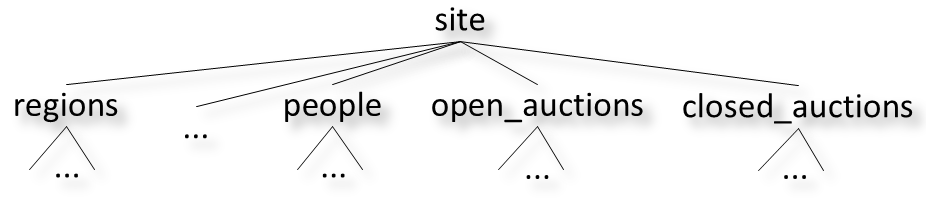
\includegraphics[width=.99\linewidth]{partialtree/figures/xmlgen1.png}
	\caption{Structure of xmlgen generated XML tree}
	\label{fig:xmlgen1}
\end{figure}


To show the effectiveness of our parallel XPath query algorithm, we
perform two types of tests. In the first test, we applied queries to an XML file of 669 MB
to show the scalability of the algorithm with respect to the number of PCs.
In the second test, we fixed the number of PCs to 16 and increased the size of the XML documents.
 
\begin{table*}[t]
	\caption{Queries used for the experiments}
	\label{table:queries}
	\centering\begin{tabular}{l|l}
		\hline
		Q4 & \texttt{/child::site/descendant::keyword/parent::text}\\
		Q5 & \texttt{/child::site/child::people/child::person[child::profile/child::gender]/child::name} \\
		Q6 & \texttt{/child::site/child::open\_auctions/child::open\_auction/child::bidder[following-sibling::bidder]} \\
		Q7 & \texttt{/child::site/child::closed\_auctions/child::closed\_auction/child::annotation/child::description/}\\
		& \hfill\texttt{child::text/child::keyword} \\
		\hline
	\end{tabular}
\end{table*}


We use the queries in Table~\ref{table:queries} for our tests.  The
first three queries Q4, Q5, and Q6 test the scalability and
data processing ability.  The last Q7, which has the most steps, is to
test how much the network communications affect the performance.


\subsection{Hardware}

The algorithm was implemented under a server/client architecture 
programmed in Java. The server ran on a single PC, 
which has an Intel(R) Core(TM) i5-760 CPU @ 2.80 GHz CPU, 8 GB of memory, 
and the OS and Java environment are Windows 7 and Java 1.8. 
The clients ran on at most 16 PCs in a PC cluster, where 
9 PCs have Intel(R) Core(TM) i5-2500 @ 3.30 GHz CPU, 7 PCs have Intel(R) have Core(TM) 
i5 CPU 760 @ 2.80GHz, 8 GB of memory, and the OS and Java environment are Ubuntu 14.04 LTS (Linux kernel: 3.16.0-41-generic) and Java 1.8.  
We solely focus on the performance of our algorithms querying on partial trees; 
thus, we construct only one partial tree for each client computer  
and do not use any multi-thread techniques, hyper threading, or other 
memory-sharing techniques. 



\subsection{Parallel speedups}
\label{sec:speedup}

This first experiment tested the efficiency and parallel speedups of
querying with respect to the number of PCs. We use an XML file of size
669 MB and the three queries Q4, Q5, and Q6 with 1, 2, 4, 8 and 16
client PCs. 
The size of XML data on one single computer we have tested is 669 MB. 
We split the input trees evenly by size.

\begin{figure*}[t]
	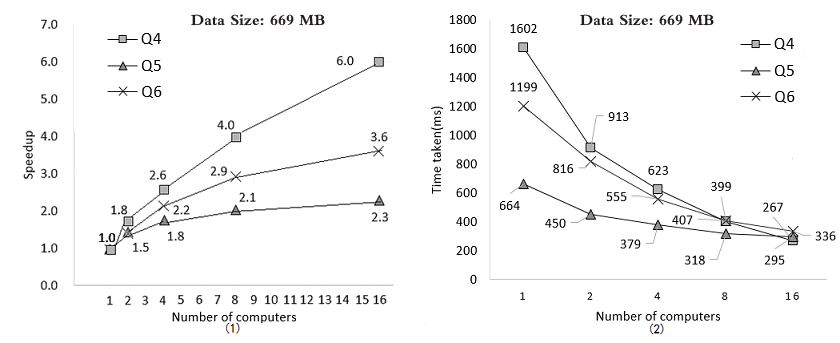
\includegraphics[width=.95\linewidth]{partialtree/figures/ex1.png}
	\caption{Speedups and time with respect to the number of clients PCs}
	\label{fig:exp-1}
\end{figure*}

Fig.~\ref{fig:exp-1} shows the speedups and time taken for the three queries.
The time taken is significantly reduced for all three queries as the number of 
clients increases.
It is more apparent for Q4. Because Q4 has no predicate and the communication affects
the overall time less. We achieved speedups of a factor of 6.0 for Q4 with 16 clients.
Both Q5 and Q6 have a predicate, and it requires more communication phases. 
The speedups for them are relatively low, a factor of 3.6 for Q6 and 2.3 for Q5.
We will discuss these lower speedups by analyzing the network communication cost in Section~\ref{sec:networkcost}.

\subsection{Scalability}
\label{sec:Scalability}

The second experiment is designed to evaluate the performance of data
processing ability per computer as the sizes of input XML data
increase. The size of XML data on a single computer that can be
processed is limited to around 669 MB because of the limit of the size of memory of a
single computer. Some necessary fields and variables of a single node
are declared, which takes extra space that is more than the size of the original XML
string. We split input data at a maximum of 512 MB for a single computer. 
We use 16 computes for
computation, and the sizes of the input XML data range from 1 GB to
8 GB. The time taken is shown in Fig.~\ref{fig:exp-2}~(1).

\begin{figure*}[t]
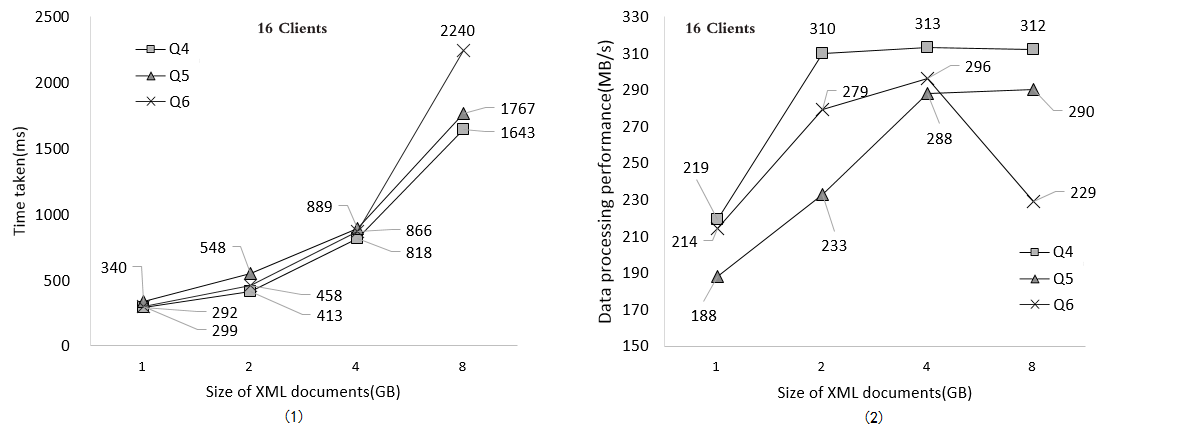
\includegraphics[width=.95\linewidth]{partialtree/figures/ex2.png}
\caption{Time taken and data processing ability}
\label{fig:exp-2}
\end{figure*}
 
The times taken of Q4 and Q5 are almost doubled as the sizes of the input XML
data doubled as shown in Fig.~\ref{fig:exp-2}~(1). For Q6, the time taken is doubled
when the size of data increases from 1 GB to 2 GB and 2 GB to 4 GB. However,
when the size of data increases from 4 GB to 8 GB, the time taken is a little
more than doubled. We believe that the extra time is likely caused by 
the cost by the rapid increase of intermediate
data and the cost of network communication. We will discuss the cost of
the network communication in the following section.

From Fig.~\ref{fig:exp-2}~(2), the data processing ability of a single
computer ranges from about 200 MB/s to 300 MB/s. We also find that when
the size of data increases, the data processing ability increases as
well. It also attributes to the cost of the network communication.



\subsection{Communication Cost}
\label{sec:networkcost}

Our algorithms are implemented with server/client architecture. 
The communication between the server and the clients is based
on TCP/IP protocol. The server is in charge of partial tree construction and 
evaluation control of queries. It holds the information of open nodes of all the partial trees,
including the ranges. The communication mechanism in our framework is based on string messages. 
We tested the communication between the server and the clients. The results
are shown in Fig.~\ref{fig:exp-3}.
 
\begin{figure*}[t]
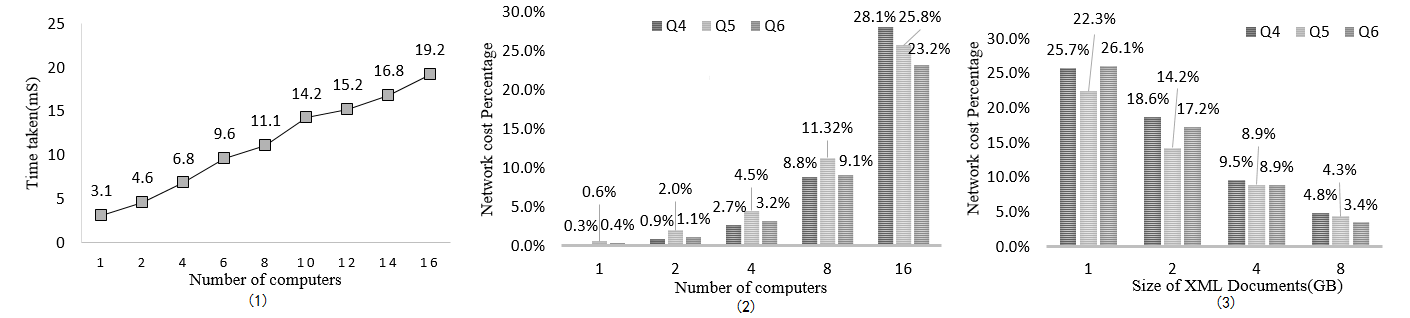
\includegraphics[width=.95\linewidth]{partialtree/figures/ex3.png}
\caption{Cost of network communication}
\label{fig:exp-3}
\end{figure*}

As we can see in Fig.~\ref{fig:exp-3}~(1), when a new client is added,
it takes approximately 1 extra millisecond for a single step on the network. 
For 16 clients, each query step takes around 20 ms for network
communication. We also tested Q7. Even if we use more computers, we obtain a
speedup of less than 1, which means the efficiency is slowed down by the
cost of network communication.

For Q7, the efficiency goes down even when the number of clients
increases. The reason is that for each step of the Q7, it takes around
20 ms for the communication when 16 clients are used. In addition, the
child axis does not take too much time for evaluation. Therefore, the
time saved by increasing the number of clients is wasted due to the cost of
network communication.

We also evaluated the cost of network communication for the former two
experiments. 
For the experiments in Section~\ref{sec:speedup}, as we can
see in Fig.~\ref{fig:exp-3}~(2), the more computers are used, the more
time is taken on network communication.  That is why the speedup increase 
was not obvious when more computers were added.  We can obtain the
same conclusion from Fig.~\ref{fig:exp-3}~(3).  

For the experiments in this section, since the number of computers are the same,
the time taken on network is almost the same. When the size of the
data increases, the effect of network communication becomes
less. Therefore, we can conclude that we can obtain better performance as
the size of the data increases. For the network, if we could improve the 
implementation to reduce the cost of network communication, 
we could get better performance for a small amount of data.

\subsection{Imbalance of Xmlgen-generated XML tree}
After analyzing these data carefully, we find that our 
algorithm does not show the best performance by using these XML documents,
because of the imbalanced structure of xmlgen-generated XML documents. 

In Fig.~\ref{fig:xmlgen1}, the children of the root have different tags. 
When we evaluate an XPath query on this tree by using 
our algorithm, we sometimes only query a small part of the tree, which means we apply queries 
on some of the partial trees that contain specific nodes while we do nothing to the others partial trees. 

For example, as we can see in Fig.~\ref{fig:xmlgen2}, the highlighted parts
are the traversed edges of the tree by Q7. We use two computers for the query. 
The specific nodes are all on the first partial tree on computer 1. 
While on computer 0, there is no node that has the tag name "\texttt{close\_auction}" 
as child of \texttt{site}; therefore, computer 1 is idle after testing the second step of Q7. 

From our experiments, we also find that only part of the computers take part in the computation. 
When we use only one computer for loading 669 MB of data, the total number of nodes is 10023967. And there are 
15300 \texttt{person} nodes for Q5 and 72000 \texttt{closed\_auction} nodes for Q6.
As we can see in Table ~\ref{table:discussionexp16} and ~\ref{table:discussionexp4}, 
we only obtain 2 out of PCs 4 and 3 out of 16 PCs that have a result node after
processing \texttt{/child::person} in Q5. That means only a few of the PCs are used in the query while the others are idle. 
We also notice that when the number of computers increased from 4 to 16, 
the us of the computers for computation only increased from 2 to 3 for \texttt{child::people}.
Thus, we cannot utilize the total number of PCs. We can obtain the same 
conclusion when we take a look at the data for processing \texttt{/child::close\_auction} step in Q6. 

One more thing we have noticed is the imbalance of nodes distribution of partial trees. 
Note that for PC$_9$ or PC$_1$$_0$, there are almost three times more nodes compared to others.
Due to the fact that we need to wait until all the computers' work is done for the next step, 
the imbalanced distribution of nodes also reduces the speedup of these experiments. 
 
From the above discussion, we come to the conclusion that the structure 
of input XML documents affects the speedups of the experiments. 
If we apply our algorithm to some well-balanced XML trees, 
we could obtain better speedups related to the increase in the number of computers.


\begin{table}[t]
	\caption{16 PCs are used for steps in Q5 and Q6.}
	\label{table:discussionexp16}
	\centering
	\begin{tabular}{c|c|c|c}
		\hline
		\hline
	 PC id	& Nodes Count	& /person & /open\_auctions \\ 		
		\hline 
		1 &	442240	& 0	& 0  \\ 
		\hline 	
		2 &	444828		& 0	& 0  \\ 
		\hline 	
		3 &	442158		& 0	& 0  \\ 
		\hline 		
		4 &	444515		& 0	& 0  \\ 
		\hline 		
		5 &	441671		& 0	& 0  \\ 
		\hline 		
		6 &	442697		& 0	& 0  \\ 
		\hline 		
		7 &	442021		& 0	& 0  \\ 
		\hline 	
		8 &	546640 &	14247 & 0	\\
		\hline
		9 &	1331617 &	102551 & 0	\\
		\hline
		10 & 1042920	& 36204	& 12032 \\
		\hline
		11 &	886279	&0	& 18666 \\
		\hline
		12 &	890306  & 0 &	18643 \\
		\hline
		13 & 891300		& 0 & 18720 \\
		\hline
		14 &	591080	& 0	& 3943 \\
		\hline
		15 &	513317	& 0 & 0	\\
		\hline
		16 &	230460	& 0 & 0	 \\
		\hline 
	\end{tabular}
\end{table}

\begin{table}[t]
	\caption{4PCs are used for steps in Q5 and Q6}
	\label{table:discussionexp4}
	\centering
	\begin{tabular}{c|c|c|c}
		\hline
		\hline
		PC id	& Nodes Count	& /person & /open\_auctions \\ 		
		\hline 
		1 &	1773703	& 0	& 0  \\ 
		\hline 	
		2 &	1872954		& 14242	& 0  \\ 
		\hline 	
		3 &	4151158		& 138759	& 49338  \\ 
		\hline 		
		4 &	2226168		& 0	& 22663  \\ 
		\hline
	\end{tabular}
\end{table}


\begin{figure}[t]
	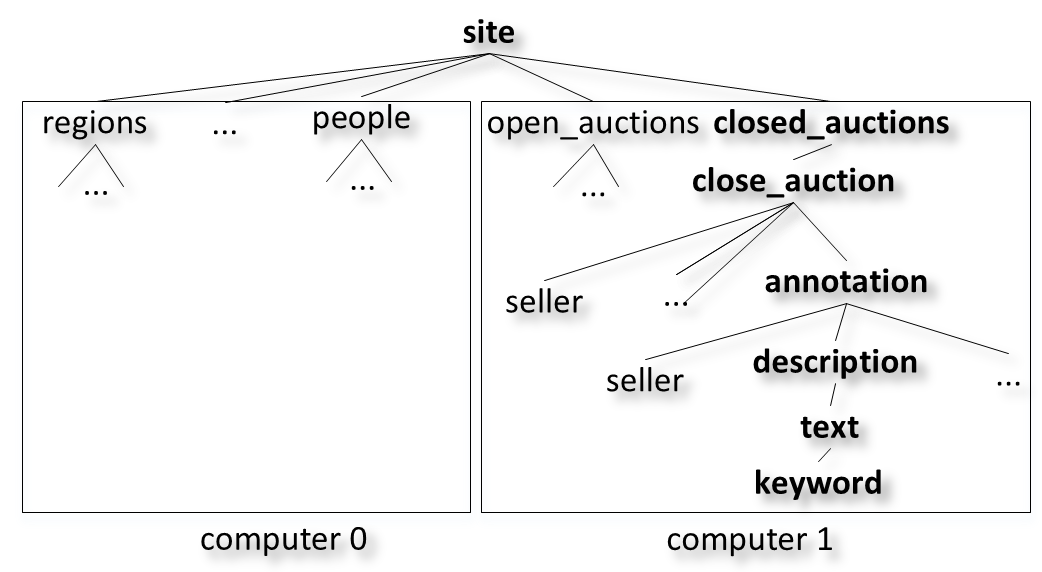
\includegraphics[width=.99\linewidth]{partialtree/figures/xmlgen2.png}
	\caption{An example of tree assignment to computers}
	\label{fig:xmlgen2}
\end{figure}

% LocalWords: kmatsu LTS xmlgen XMark scalability TCP IP

\section{Related Work}

Many papers have addressed the topic of implementations of XPath queries 
in parallel. One significant paper was presented by IBM~\cite{BLKK09}. The paper 
proposes three kinds of strategies for XPath queries in 
parallel: data partition strategy, query partition strategy, 
and hybrid partition strategy. Many papers can be categorized to one of the strategies. \cite{KrYa10,ZhPC10,HSYW14} focus on XPath queries 
implemented in a shared-memory environment. \cite{PLZC07,WZYL08}
focused on XML parsing, which is related to our parsing 
algorithm. \cite{AnAH10} proposed ideas about XML processing 
techniques that are helpful for our research. 
Some prior researches are based on a common assumption 
that a large amount of XPath queries are executed over an XML stream.
YFilter\cite{DiFF11} and XMLTK \cite{AvGT02} execute thousands of small queries in parallel. The parsing phase is still sequential.
Indexing is also a hot topic for improving the performance of parallel XML queries processing.
\cite{CVZT02}, \cite{Grus02}, \cite{JLCW02} are related to this field. 
They examined the indices on different types of trees, including B+-tree, R-tree, and XR-tree. 

The idea of dividing the XML documents and running the computation for trees
with the chunks is not new.   Kakehi et al.~\cite{KaME07} showed a parallel tree reduction algorithm
from the nodes in chunks.  Based on the idea given by Kakehi et al., Emoto and Imachi~\cite{EmIm12} developed 
a parallel tree reduction algorithm on Hadoop, and Matsuzaki and Miyazaki~\cite{MaMi15} developed 
a parallel tree accumulation algorithm. A similar approach was taken by Sevilgen et al.~\cite{SeAF05} who developed a simpler version of tree accumulations over the serialized representation of trees.

It is known that we can develop a parallel algorithm for XPath queries using the tree accumulations~\cite{Mats07}.
The approach we took in this paper is inspired by the work by Morihata~\cite{Mori13}.
To discuss the advantages of the proposed algorithm and compare by implementation with other approaches
are our important future work.


\section{Conclusion}

In this paper, we proposed algorithms for a subset of 
XPath queries on a large XML tree in parallel and 
implemented them on a 16-node PC cluster. 
We developed our own framework for the experiments. The 
experiment results showed a speedup of a factor of 6 on a 16-node PC cluster. 

\paragraph*{Acknowledgments}
Part of this work was supported by JSPS KAKENHI No. 25330088.


\begin{thebibliography}{99}
\bibitem{AnAH10}
Andriescu E.-M., Azzabi A., Hains G. Parallel 
processing of Forward XPath queries: an experiment 
with BSML, \emph{TR-LACL} Vol 11, 2010 
\bibitem{AvGT02}
Avila-Campillo I., Green T. J., et al. XMLTK: An
XML toolkit for scalable XML stream processing.
\emph{Technical report, PlanX}, 2002.
\bibitem{BLKK09}
Bordawekar, R., Lim, L., Kementsietsidis, A., Kok, 
B., To Parallelize or Not to Parallelize: XPath 
Queries on Multi-core Systems, \emph{IBM Research 
Report}, 2009 
\bibitem{CVZT02}
Chien S.Y., Vagena Z., Zhang D., Tsotras V. J., Zaniolo C.,Efficient 
Structural Joins on Indexed XML Documents. \emph{VLDB 2002}, pp.263--274, 2002,
\bibitem{DiFF11}
Diao Y., Fischer P., Franklin M., et al. YFilter:
Efficient and scalable filt. of XML doc. In ICDE,
pages 341--342, 2002.
\bibitem{EmIm12}
Emoto, K., Imachi, H.: Parallel tree reduction on {MapReduce}.
In \emph{Proceedings of the International Conference
  on Computational Science} (\emph{ICCS 2012}),
  \emph{Procedia Computer Science}, vol.~9, pp. 1827--1836. Elsevier, 2012.
\bibitem{xpathcategory}
Franceschet M., XPathMark: Functional and performance tests for XPath.
In \emph{XQuery Implementation Paradigms}, Dagstuhl Seminar Proceedings No. 06472, Internationales Begegnungs- und Forschungszentrum f{\"u}r Informatik (IBFI), Schloss Dagstuhl, Germany, 2007.
\bibitem{FrDa11}
Francis N., David C., and Libkin L., A direct
transation from XPath to nondet. automata. \emph{In
Workshop on Foundations of Data Management}, pp.350--361, 2011
\bibitem{mbridges1}
Gazit H., Miller G.L., Teng S.-H., Optimal tree contraction in EREW model, \emph{Proceedings of the Princeton Workshop on Algorithms, Architectures, and Technical Issues for Models of Concurrent Computation}, pp.139-156, 1987
\emph{APLAS}, 2002
\bibitem{Grus02}
Grust T., Accelerating XPath Location Steps. \emph{SIGMOD 2002}, pp.109--120, 2002
\bibitem{HSYW14}
Huang X., Si X., Yuan X., Wang C., A Dynamic 
Load-balancing Scheme for XPath Queries Parallelization 
in Shared Memory Multi-core Systems, 
\emph{Journal of Computers}, pp.1436--1445, 2014 
\bibitem{JLCW02}
Jiang H.F., Lu H.J., Chin B., Wang W., XR-Tree:Indexing XML Data for 
Efficient Structural Joins. \emph{ICDE}, pp.253--264, 2003
\bibitem{KaME07}
Kakehi, K., Matsuzaki, K., Emoto, K.,
Efficient Parallel Tree Reductions on Distributed Memory Environments.
\emph{7th International Conference on Computational Science} (\emph{ICCS2007}), pp.601--608, 2007.
\bibitem{mbridges}
Kawamura K., Matsuzaki K., Dividing Huge XML Trees Using the m-bridge Technique over One-to-one orresponding Binary Trees. \emph{IPSJ Transaction on Programming}, pp.40--50, 2014. 
\bibitem{KrYa10}
Krulis, E., Yaghob, E., Efficient Implementation of 
XPath Processor on Multi-Core CPUs,  pp. 60--71, 
2010 
\bibitem{Mats07}
Matsuzaki, K., Parallel Programming with Tree Skeleton.
Ph.D. Thesis, The University of Tokyo, 2007.
\bibitem{MaMi15}
Matsuzaki, K., Miyazaki, R., 
Parallel Tree Accumulations on MapReduce.
\emph{International Journal of Parallel Programming}, online, 2015.
\bibitem{Mori13}
Morihata, A. Work Efficient Distributed-Memory Parallel Evaluation of XPath Queries,
In \emph{30th JSSST Conference Proceedings}, 2013. (in Japanese).
\bibitem{PLZC07}
Pan, Y., Lu, W., Zhang, Y., Chiu, K., A static 
load-balancing scheme for parallel XML parsing on 
multicore CPUs. \emph{IEEE International Symposium on 
Cluster Computing and the Grid}, Janeiro, pp. 
351--362, 2007 
\bibitem{SeAF05}
Sevilgen, F.E., Aluru, S., Futamura, N., Parallel Algorithms for Tree Accumulations,
\emph{Journal of Parallel and Distributed Computing}, vol.~65, no.~1, pp.85--93, 2005.
\bibitem{XML}
W3C, XML Tutorial, http://www.w3schools.com/xml/, 2010. 
\bibitem{XPath}
W3C, XML Path Language (XPath) 2.0 (Second 
Edition), http://www.w3.org/TR/xpath20/, 2010. 
\bibitem{WZYL08}
Wu, Y., Zhang, Q., Yu, Z., Li, J. A Hybrid Parallel 
Processing for XML Parsing and Schema Validation. 
\emph{The Markup Conference, Cluster Computing and the 
Grid, Seventh IEEE International Symposium}, pp. 
351--362, 2008. 
\bibitem{XMark}
XMark, XMark - An XML Benchmark Project, 
http://www.xml-benchmark.org/generator.html, 2010. 
\bibitem{ZhPC10}
Zhang, Y., Pan Y., Chiu K., A Parallel XPath Engine 
Based on Concurrent NFA Execution, \emph{IEEE 16th 
International Conference on Parallel and Distributed 
Systems}, pp. 314--321, 2010 
\end{thebibliography}


\begin{biography}

\profile{Wei Hao}{is a Ph.D. student in Kochi University of Technology in Japan and is a Lecture in Anhui University of Science and Technology in China. 
	He received his B.E. and M.S. from Anhui University of Science and Technology in 2004 and 2007, respectively, and began doctoral study since 2014. 
	His current research interest is in parallel programming and XML data processing. }
%
\profile{Kiminori Matsuzaki}{is an Associate Professor of Kochi
  University of Technology in Japan.  He received his B.E., M.S. and
  Ph.D. from The University of Tokyo in 2001, 2003 and 2007,
  respectively.  He was an Assistant Professor (2005--2009) in The
  University of Tokyo, before joining Kochi University of Technology
  as an Associate Professor in 2009.  His research interest is in
  parallel programming and algorithm derivation. He is a member of
  ACM, JSSST, IEEE\@.}
%
\end{biography}

\end{document}


